\documentclass[11pt, serbianc, english, titlepage]{article}

\usepackage[utf8]{inputenc}
\usepackage[T2A]{fontenc}
\usepackage[main=serbianc]{babel}
\usepackage{amsmath}
\usepackage{amsfonts}
\usepackage{amssymb}
\usepackage{graphicx}
\usepackage[left=1in,right=1in,top=1in,bottom=1in]{geometry}
\usepackage{listings}
\usepackage[official]{eurosym}
\usepackage{color}
\usepackage{xcolor}
\usepackage{blkarray}
\usepackage{makeidx, multicol}\makeindex
\usepackage{url}
\usepackage{caption}
\usepackage[autostyle]{csquotes}
\usepackage{textcomp}
\usepackage{setspace}
\usepackage[bottom]{footmisc}


\usepackage[unicode,  bookmarks]{hyperref}
\hypersetup{hyperindex=true, colorlinks=true,linkcolor=black, citecolor=red, }

\DeclareCaptionFont{white}{\color{white}}
\DeclareCaptionFormat{listing}{\colorbox{gray}{\parbox{\textwidth}{#1#2#3}}}
\captionsetup[lstlisting]{format=listing,labelfont=white,textfont=white}
\interfootnotelinepenalty=10000
%\bibpunct{[}{]}{;}{a}{,}{,}


\addto\captionsserbianc{\renewcommand{\indexname}{Индекс појмова}}
\addto\captionsserbianc{\renewcommand{\contentsname}{Садржај}}
\renewcommand{\lstlistingname}{К\^{о}д}
\newcommand{\sidenote}[1]{%
        \refstepcounter{sidenote}\mbox{\textsuperscript{\alph{sidenote}}}%
        \marginpar{\footnotesize \mbox{\textsuperscript{\alph{sidenote}} }#1}%
}
\newcounter{sidenote}

\lstset{language=Python, framexleftmargin=5mm, frame=none,
captionpos = b, showstringspaces=false}
\renewcommand\lstlistlistingname{Програмски к\^{о}дови}

\hfuzz=20pt
\vfuzz=20pt
\hbadness=2000
\vbadness=\maxdimen





\begin{document}

%%%%%%%%%%%%%%%%%%%%%%%%%%%%%%%%%%%%%%%%%
% University Assignment Title Page 
% LaTeX Template
% Version 1.0 (27/12/12)
%
% This template has been downloaded from:
% http://www.LaTeXTemplates.com
%
% Original author:
% WikiBooks (http://en.wikibooks.org/wiki/LaTeX/Title_Creation)
%
% License:
% CC BY-NC-SA 3.0 (http://creativecommons.org/licenses/by-nc-sa/3.0/)
% 
% Instructions for using this template:
% This title page is capable of being compiled as is. This is not useful for 
% including it in another document. To do this, you have two options: 
%
% 1) Copy/paste everything between \begin{document} and \end{document} 
% starting at \begin{titlepage} and paste this into another LaTeX file where you 
% want your title page.
% OR
% 2) Remove everything outside the \begin{titlepage} and \end{titlepage} and 
% move this file to the same directory as the LaTeX file you wish to add it to. 
% Then add %%%%%%%%%%%%%%%%%%%%%%%%%%%%%%%%%%%%%%%%%
% University Assignment Title Page 
% LaTeX Template
% Version 1.0 (27/12/12)
%
% This template has been downloaded from:
% http://www.LaTeXTemplates.com
%
% Original author:
% WikiBooks (http://en.wikibooks.org/wiki/LaTeX/Title_Creation)
%
% License:
% CC BY-NC-SA 3.0 (http://creativecommons.org/licenses/by-nc-sa/3.0/)
% 
% Instructions for using this template:
% This title page is capable of being compiled as is. This is not useful for 
% including it in another document. To do this, you have two options: 
%
% 1) Copy/paste everything between \begin{document} and \end{document} 
% starting at \begin{titlepage} and paste this into another LaTeX file where you 
% want your title page.
% OR
% 2) Remove everything outside the \begin{titlepage} and \end{titlepage} and 
% move this file to the same directory as the LaTeX file you wish to add it to. 
% Then add %%%%%%%%%%%%%%%%%%%%%%%%%%%%%%%%%%%%%%%%%
% University Assignment Title Page 
% LaTeX Template
% Version 1.0 (27/12/12)
%
% This template has been downloaded from:
% http://www.LaTeXTemplates.com
%
% Original author:
% WikiBooks (http://en.wikibooks.org/wiki/LaTeX/Title_Creation)
%
% License:
% CC BY-NC-SA 3.0 (http://creativecommons.org/licenses/by-nc-sa/3.0/)
% 
% Instructions for using this template:
% This title page is capable of being compiled as is. This is not useful for 
% including it in another document. To do this, you have two options: 
%
% 1) Copy/paste everything between \begin{document} and \end{document} 
% starting at \begin{titlepage} and paste this into another LaTeX file where you 
% want your title page.
% OR
% 2) Remove everything outside the \begin{titlepage} and \end{titlepage} and 
% move this file to the same directory as the LaTeX file you wish to add it to. 
% Then add \input{./title_page_1.tex} to your LaTeX file where you want your
% title page.
%
%%%%%%%%%%%%%%%%%%%%%%%%%%%%%%%%%%%%%%%%%

%----------------------------------------------------------------------------------------
%	PACKAGES AND OTHER DOCUMENT CONFIGURATIONS
%----------------------------------------------------------------------------------------




\begin{titlepage}

\newcommand{\HRule}{\rule{\linewidth}{0.5mm}} % Defines a new command for the horizontal lines, change thickness here

\center % Center everything on the page
 
%----------------------------------------------------------------------------------------
%	HEADING SECTIONS
%----------------------------------------------------------------------------------------

\textsc{\LARGE Математички факултет у Београду}\\[1.5cm] % Name of your university/college
\textsc{\Large Мастер рад}\\[0.5cm] % Major heading such as course name
%\textsc{\large Minor Heading}\\[0.5cm] % Minor heading such as course title

%----------------------------------------------------------------------------------------
%	TITLE SECTION
%----------------------------------------------------------------------------------------

\HRule \\[0.4cm]
{ \huge \bfseries Примена програмског језика Python \\[0.1cm]
 у реализацији алгоритама за \\[0.3cm]
 рангирање веб страница}\\[0.4cm] % Title of your document
\HRule \\[1.5cm]
 
%----------------------------------------------------------------------------------------
%	AUTHOR SECTION
%----------------------------------------------------------------------------------------

\begin{minipage}{0.4\textwidth}
\begin{flushleft} \large
\emph{Аутор:}\\
Игор \textsc{Илић} % Your name
\end{flushleft}
\end{minipage}
~
\begin{minipage}{0.4\textwidth}
\begin{flushright} \large
\emph{Ментор:} \\
Проф. др Владимир \textsc{Филиповић} % Supervisor's Name
\end{flushright}
\end{minipage}\\[4cm]

% If you don't want a supervisor, uncomment the two lines below and remove the section above
%\Large \emph{Author:}\\
%John \textsc{Smith}\\[3cm] % Your name

%----------------------------------------------------------------------------------------
%	LOGO SECTION
%----------------------------------------------------------------------------------------


\includegraphics[scale=0.33]{vecigrb.png} \\[1cm]  %Include a department/university logo - this will require the graphicx package

%----------------------------------------------------------------------------------------
%	DATE SECTION
%----------------------------------------------------------------------------------------

{\large Београд, \the\year}\\[3cm] % Date, change the \today to a set date if you want to be precise


 
%----------------------------------------------------------------------------------------

\vfill % Fill the rest of the page with whitespace

\end{titlepage}
 to your LaTeX file where you want your
% title page.
%
%%%%%%%%%%%%%%%%%%%%%%%%%%%%%%%%%%%%%%%%%

%----------------------------------------------------------------------------------------
%	PACKAGES AND OTHER DOCUMENT CONFIGURATIONS
%----------------------------------------------------------------------------------------




\begin{titlepage}

\newcommand{\HRule}{\rule{\linewidth}{0.5mm}} % Defines a new command for the horizontal lines, change thickness here

\center % Center everything on the page
 
%----------------------------------------------------------------------------------------
%	HEADING SECTIONS
%----------------------------------------------------------------------------------------

\textsc{\LARGE Математички факултет у Београду}\\[1.5cm] % Name of your university/college
\textsc{\Large Мастер рад}\\[0.5cm] % Major heading such as course name
%\textsc{\large Minor Heading}\\[0.5cm] % Minor heading such as course title

%----------------------------------------------------------------------------------------
%	TITLE SECTION
%----------------------------------------------------------------------------------------

\HRule \\[0.4cm]
{ \huge \bfseries Примена програмског језика Python \\[0.1cm]
 у реализацији алгоритама за \\[0.3cm]
 рангирање веб страница}\\[0.4cm] % Title of your document
\HRule \\[1.5cm]
 
%----------------------------------------------------------------------------------------
%	AUTHOR SECTION
%----------------------------------------------------------------------------------------

\begin{minipage}{0.4\textwidth}
\begin{flushleft} \large
\emph{Аутор:}\\
Игор \textsc{Илић} % Your name
\end{flushleft}
\end{minipage}
~
\begin{minipage}{0.4\textwidth}
\begin{flushright} \large
\emph{Ментор:} \\
Проф. др Владимир \textsc{Филиповић} % Supervisor's Name
\end{flushright}
\end{minipage}\\[4cm]

% If you don't want a supervisor, uncomment the two lines below and remove the section above
%\Large \emph{Author:}\\
%John \textsc{Smith}\\[3cm] % Your name

%----------------------------------------------------------------------------------------
%	LOGO SECTION
%----------------------------------------------------------------------------------------


\includegraphics[scale=0.33]{vecigrb.png} \\[1cm]  %Include a department/university logo - this will require the graphicx package

%----------------------------------------------------------------------------------------
%	DATE SECTION
%----------------------------------------------------------------------------------------

{\large Београд, \the\year}\\[3cm] % Date, change the \today to a set date if you want to be precise


 
%----------------------------------------------------------------------------------------

\vfill % Fill the rest of the page with whitespace

\end{titlepage}
 to your LaTeX file where you want your
% title page.
%
%%%%%%%%%%%%%%%%%%%%%%%%%%%%%%%%%%%%%%%%%

%----------------------------------------------------------------------------------------
%	PACKAGES AND OTHER DOCUMENT CONFIGURATIONS
%----------------------------------------------------------------------------------------




\begin{titlepage}

\newcommand{\HRule}{\rule{\linewidth}{0.5mm}} % Defines a new command for the horizontal lines, change thickness here

\center % Center everything on the page
 
%----------------------------------------------------------------------------------------
%	HEADING SECTIONS
%----------------------------------------------------------------------------------------

\textsc{\LARGE Математички факултет у Београду}\\[1.5cm] % Name of your university/college
\textsc{\Large Мастер рад}\\[0.5cm] % Major heading such as course name
%\textsc{\large Minor Heading}\\[0.5cm] % Minor heading such as course title

%----------------------------------------------------------------------------------------
%	TITLE SECTION
%----------------------------------------------------------------------------------------

\HRule \\[0.4cm]
{ \huge \bfseries Примена програмског језика Python \\[0.1cm]
 у реализацији алгоритама за \\[0.3cm]
 рангирање веб страница}\\[0.4cm] % Title of your document
\HRule \\[1.5cm]
 
%----------------------------------------------------------------------------------------
%	AUTHOR SECTION
%----------------------------------------------------------------------------------------

\begin{minipage}{0.4\textwidth}
\begin{flushleft} \large
\emph{Аутор:}\\
Игор \textsc{Илић} % Your name
\end{flushleft}
\end{minipage}
~
\begin{minipage}{0.4\textwidth}
\begin{flushright} \large
\emph{Ментор:} \\
Проф. др Владимир \textsc{Филиповић} % Supervisor's Name
\end{flushright}
\end{minipage}\\[4cm]

% If you don't want a supervisor, uncomment the two lines below and remove the section above
%\Large \emph{Author:}\\
%John \textsc{Smith}\\[3cm] % Your name

%----------------------------------------------------------------------------------------
%	LOGO SECTION
%----------------------------------------------------------------------------------------


\includegraphics[scale=0.33]{vecigrb.png} \\[1cm]  %Include a department/university logo - this will require the graphicx package

%----------------------------------------------------------------------------------------
%	DATE SECTION
%----------------------------------------------------------------------------------------

{\large Београд, \the\year}\\[3cm] % Date, change the \today to a set date if you want to be precise


 
%----------------------------------------------------------------------------------------

\vfill % Fill the rest of the page with whitespace

\end{titlepage}

%\maketitle


\newpage
\pagenumbering{roman}
\tableofcontents
\newpage
\pagenumbering{arabic}

\section{Увод}
         Током развоја Интернета и поготово од настанка веба, повећавала се потреба за претраживањем страница које су биле постављене на Интернет. Са настанком веба и његовим ширењем та потреба се продубила због огромног броја информација које су преплавиле веб од настанка до данас. Највећи проблем са којим су се корисници Интернета, да се из мора информација издвоји она која је најподеснија за корисников упит. Овај рад покушаће да реши проблем претраживања  веб страница, кроз реализацију алгоритма за рангирање веб страница у програмском језику Python. Такође, у току тог процеса, биће анализиран алгоритам за рангирање PageRank\texttrademark\ \footnote{PageRank\texttrademark\ алгоритам није јавно доступан, те ће се његова анализа свести на оно што јесте јавно доступно и на анализе других аутора, нпр. \cite{langville2011google}  }  и његове предности у односу на претраживање без примене датог алгоритма.\\
         Рад ће бити подељен на неколико делова. У првом делу биће укратко објашњена синтакса и рад програмског језика Python. Обратиће се посебна пажња на основне елементе Python-а, као и на начин писања програма у њему. Такође, уз навођење једноставних примера, биће обрађени и типови података који се користе у Python-у, начин на који се уводе услови, петље, функције и модули, као и на који начин Python приступа класама и објектима.\\
         После дела о програмском језику Python биће приложен део о претраживању Интернета и обради хипервеза. Биће приложен и пример како се из HTML к\^{о}да издвајају хипервезе, што ће чинити основу веб-паука.\\
         Затим се завршава веб-паук, који скупља све хипервезе на веб страници и затим следи те хипервезе да би наставио свој процес унедоглед или до дубине претраживања који му се одреди. \\
         После тога долази се до корисниковог упита и како ће претраживач одговарати на упите. Поставља се питање да ли је могуће то радити на бржи начин и даје се одговор у облику хеш табеле.
         На крају, рад се бави питањем рангирања веб страница у процесу претраживања. Анализира се алгоритам PageRank\texttrademark\ даје се могуће решење овог алгоритма у програмском језику Python.\\
         После закључка, дати су и додаци у којима се може погледати комплетан к\^{о}д, затим поређење резултата приликом задавања модела претраживања са и без укљученог модула за рангирање страница. Такође, дат је списак програмских к\^{о}дова који су се појавили током писања овог рада, као и литература која је коришћена током писања рада.\\
         У примерима који се налазе у мастер раду је коришћена верзија Python-а 2.7.6, мада би скоро сви примери требали да раде и са новим верзијама. Примери су тестирани у програмском окружењу \emph{Eclipse}, са додатком \emph{PyDev}, а у оквиру оперативног система LinuxMint.  
          
\pagebreak
\section{Програмски језик Python}
		\subsubsection{Програмски језици и програмирање}
		Програмирање подразумева активност \emph{програмера} усмерена ка решавању конкретног проблема на рачунару. Проблем се обично решава конструкцијом \emph{алгоритма}\index{algoritam@алгоритам} за решење проблема, а алгоритам се записује посредством програмског језика. Програмски језик има улогу да обезбеди конструкције и начине за израчунавање на рачунару. Организовано израчунавање обично називамо \emph{програмом}.\\
		Програмски језик\index{Programski jezik@Програмски језик} је средство за писање програма и саопштавање програма рачунару. То је вештачки језик који првенствено служи за комуникацију између човека и рачунара, мада се понекад програмски језик користи и за комуникацију између људи.\\
		 		До сада је направљено неколико хиљада програмских језика и потребно је да се на неки начин разврстају. Постоје разне класификације, зависно од \emph{критеријума класификације}:
		\begin{itemize}
		\item степен зависности од рачунара
		\item време настанка и својства
		\item област примене
		\item начин решавања проблема
		\end{itemize}
		Тако по степену зависности од рачунара програмске језике можемо поделити на машински зависне (Асемблерски језици, Макро-језици, итд.) и машински независне програмске језике.\\
		По областима примене програмске језике можемо поделити на оне за учење програмирања (Pascal, Basic, Logo, итд.), програмске језике за развој системског софтвера (C, Asembler, итд.), за пословну примену (COBOL, SQL, ...), за развој програма на интернету (Java, Java Script, Perl, итд.), за примену у математици, и друго.\\
		Програмске језике делимо и по начину решавања проблема и то на процедуралне и непроцедуралне. Док би их по времену настанка и својствима поделили на језике I генерације (машински и асемблерски), II генерације (FORTRAN, COBOL, LISP, BASIC,...), III генерације (Pascal, C, PROLOG, Smalltalk, C++, Java, ...) и језике IV генерације (SQL, VisualBasic, сви језици унутар апликација).\cite{tosic}\\
		Може се поставити и питање \emph{зашто} учити компјутерско програмирање? Програмирање развија креативност, логичко размишљање и способност решавања проблема. Програмер добија прилику да креира \emph{нешто} из \emph{ничега}, користи логику да претвори скупове речи у компјутерски програм и кад нешто не иде како треба на дело долази способност да се реши проблем и да се нађе и исправи грешка. \\
		Програмирање је и забава. Понекад је то и захтевна (и с времена на време фрустрирајућа) активност, али где се те способности могу искористити како у школи и на послу, тако и у кући невезано за захтеве каријере и образовања.\\
		
		\subsubsection{Зашто Python?}
		Чињеница је да постоје на хиљаде програмских језика. Неки од њих су поменути у претходном делу. Шта то издваја програмски језик Python\index{Python} од других и зашто би се неко одлучио да програмира у Python-у, уместо, на пример, у Pascal-у?\\
		Python је лак за учење, а уз то има заиста корисна својства за програмера почетника. К\^{о}д је врло разумљив за читање, ако се упореди са осталим програмским језицима. Такође, постоје разни додаци (модули) који ће проширити Python на захтевани начин, тако да Python може да послужи за креирање једноставних анимација са додатком Turtle (инспирисан Turtle graphics, коришћеним у програмском језику Logo у шездесетим годинама прошлог века)\cite{briggs2012python}. Други модули служе да користимо Python као скрипт језик или као додатак разним комплекснијим језицима попут  C/C++. \\
		Надаље, Python може представљати сјајно оруђе за учење основних појмова програмирања, типова података, услова, петљи, за учење разних алгоритама(на пример сортирања), онда за имплементацију математичких формула и начина на који се те формуле могу програмирати (итеративно или рекурзивно, на пример за факторијел).\\
		Важан фактор је такође и \emph{доступност} Python-a, јер се интерпретатор може врло једноставно преузети са интернета и инсталирати на рачунару. Постоје и разне варијанте Python интерпретатора које се налазе на појединим веб страницама. Python може да ради на многобројним оперативним системима: Windows-у, Mac OS-у, Linux-у, па и на мобилним платформама iOS-у или на Android оперативном систему\cite{pythonsite} . 
		\subsubsection{Историјат и начин коришћења}
		Програмски језик Python\index{Python} је настао почетком '90-их година прошлог века. Креирао га је Холанђанин Гвидо ван Росум (Guido van Rossum)\index{Python!Guido van Rossum} и наставио да га развија до данашњег дана, наравно уз помоћ огромне заједнице програмера широм света. Данас је актуелна верзија 3.4. Гвидо је у свету познат под надимком BDFL, што је скраћеница за \emph{Доживотни Добронамерни Диктатор}\footnote{Benevolent Dictator For Life}.\\
		Python је добио име по култној британској хумористичкој серији у продукцији BBC-а, "Летећи циркус Монти Пајтона" (\emph{Monthy Python's Flying Circus}), коју су прославили легендарни глумци и комичари попут: Ерика Ајдла, Џона Клиза, Мајкла Пелина, Грејема Чепмена, режисера Терија Гилијама и других. Снимљена као алтернативни театар апсурда, серија је остала позната и у данашње време и до данас се памте и радо гледају скечеви попут "\emph{Министарства смешног ходања}", "\emph{Најсмешнији виц на свету}", итд.\\
		Оно што је још остало je да се опише на који начин може да се користи Python на рачунару. Дакле, потребан је Python интерпретатор, који се може бесплатно преузети са званичне Python-ове веб презентације\cite{pythonsite}, као и неки од текст едитора и/или развојних окружења (нпр. \emph{Eclipse} или \emph{PyCharm}) помоћу кога ће се уносити к\^{о}д. Алтернативно може се преузети и инсталирати апликација \emph{IDLE}\index{Python!IDLE@\emph{IDLE}} (\texttt{http://www.python.org/getit/} ), која омогућује да се програмира у Python-у на врло једноставан начин.\\
		\subsection{Рачунање и променљиве}
		У даљем тексту се претпоставља да је Python инсталиран на рачунару и апстрахује се начин на који се добија резултат на потенцијалном екрану или принтеру. Дакле, описује се искључиво програмски језик Python, његова синтакса, као и шта се све може да урадити помоћу њега.
		\subsubsection{Python као калкулатор}
		Python\index{Python!kalkulator@калкулатор} може да послужи и као обичан калкулатор\cite{van2003introduction,lutz2009learning}. Ако је потребно да се изврше основне аритметичке операције: сабирање, одузимање, множење и дељење, треба користити адекватне симболе за дате операције (редом): +, -, *, /. Поставља се питање како се Python односи према разним типовима бројева. Бројеви у рачунарству се обично деле на целобројне и бројеве у покретном зарезу. За операције сабирања, одузимања и множења правило је врло једноставно\index{Python!operacije@операције са бројевима}: ако се ради са целим бројевима, добија се и целобројни резултат. Исто важи и за бројеве у покретном зарезу. Мало је другачији случај са дељењем. Ако се врши дељење целих бројева, количник ће бити дат као децимални број. Ако треба да се као резултат добије цео део количника, користи се симбол "//". На пример:
\begin{lstlisting}[caption = Примери операција са бројевима, label = racun]

>>> 100 + 16
116
>>> 96.0 - 11
85.0
>>> 11.1 * 10
111.0
>>> 20/5
4.0
>>> 20 / 8
2.5
>>> 20 // 8
2
\end{lstlisting}
Moгу се користити и друге математичке операције, као што су степеновање\index{Python!stepenovanje@степеновање} или се може направити програм за произвољну математичку функцију. Степеновање је другачије него што је то у осталим програмским језицима и обавља се помоћу симбола "**":
\begin{lstlisting}[caption = Степеновање, label = stepen]
>>> 2 ** 32
4294967296
\end{lstlisting}
Такође, Python омогућава и рачунање са комплексним бројевима у алгебарском облику\jndex{Python!kompleksni@комплексни бројеви}, где се код комплексних бројева користи суфикс "j" или "J" ако треба да се назначи имагинарни део тог комплексног броја. На пример:
\begin{lstlisting}[caption = Операције са комплексним бројевима, label = kompleksni]
>>> (1+1j)*(2-1j)
(3+1j)

>>> 1j ** 2
(-1+0j)
>>> 1j * 1J
(-1+0j)
>>> 
\end{lstlisting}
		\subsubsection{Променљиве}
		Променљивој се додељује одговарајућа вредност, која може бити бројчана или логичка (тачно или нетачно) или променљива може да реферише на вредност друге променљиве. Ако је ово последње случај, промена вредности једне променљиве, утиче и на вредност друге променљиве. У примеру који следи, наредбом:
		\begin{lstlisting}
>>>a = 1
		\end{lstlisting}
		\begin{figure}[here]
		\centering
		
\includegraphics{1a.png}
		\caption{a показује на вредност 1}
		\label{slike:a_je_1}
		\end{figure}
		променљива \emph{а} има вредност 1. Може се рећи и да променљива реферише на вредност 1 која се налази негде у меморији.\\
		Ако се истој променљивој додели нека друга вредност, на пример 2, онда ће она реферисати на број 2, док је број 1 напуштен.
		\begin{lstlisting}
>>>a = 2
		\end{lstlisting}
		\begin{figure}[here]
		\centering
		
\includegraphics{2a.png}
		
\includegraphics{1.png}
		\caption{a сада показује на вредност 2}
		\label{slike:a_je_2}
		\end{figure}
		
		Потом може да се уведе нова променљива и да се подеси да реферише на променљиву \emph{а}.
		\begin{lstlisting}
>>>b = a
		\end{lstlisting}
		\begin{figure} [here]
		\centering	
		
\includegraphics{2ab.png}
		\caption{и а и b показују на исту вредност}
		\label{slike:a_b_je_2}
		\end{figure}
		Тада и једна и друга променљива реферишу на исту вредност. Ако би се једној од њих променила вредност, тада би друга реферисала на нову вредност.\\
		
		
		
		
		
		Имена променљиве се по договору пишу свим малим или свим великим словима латинице, иако Python дозвољава све начине писања променљивих, осим што нису дозвољене кључне речи. Прави Пајтонисти\footnote{Погледати: "How to think like a Pythonista", \texttt{http://python.net/crew/mwh/hacks/objectthink.html} } кажу да им је само име "променљива" неприкладно за оно што она ради у Python-у, те да би бољи избор био употребити речи: "именa",  "објекти" или "везивања" (\emph{енгл., bindings}).\\
		Променљиве се могу користити и у рачунању. На пример:
\begin{lstlisting}[caption = Пример коришћења променљивих, label = variables]
>>> br_stanovnika = 9860000 # br. stanovnika Srbije prema proceni iz 2010.
>>> povrsina = 77474 # povrsina Srbije u kv. kilometrima
>>> gustina_naseljenosti = br_stanovnika / povrsina
>>> print (gustina_naseljenosti)
127.26850298164545
\end{lstlisting}

		Дакле, могло би се рећи да програмски језик Python садржи функционалност моћног калкулатора који допушта и задавање одговарајуће вредности променљивима (именима) уз поштовање претходно наведеним правила.
		\subsection{Типови података}
		Осим бројева (целих, у покретном зарезу и других који нису обухваћени јер би иначе обим рада постао превише велики) и променљивих у Python-у постоје и типови података. То су:
		\begin{itemize}
		\item Ниске (енгл. \emph{strings})
		\item Уређене n-торке (енгл. \emph{tuples})
		\item Листе (енгл. \emph{lists})
		\item Мапе (енгл. \emph{dictionary})
		\end{itemize}
		Ови типови података могу бити мутабилни (променљиви) и немутабилни (непроменљиви). Тако су листе и речници мутабилни, док су уређене n-торке и ниске непроменљиви. То значи да се, на пример листа која је задата једној променљивој може трајно променити коришћењем наредби и поступака које ће касније бити описане, док рецимо уређене n-торке не могу да се мењају већ само може да се користи њихов садржај.
		\subsubsection{Ниске}
		Ниска\index{Python!string@стринг} је заправо текст, односно може се размишљати о нисци као секвенци слова. Тако сва слова, бројеви и специјални знаци из овог рада, могу чинити једну ниску. Да би се креирала ниска потребно је поставити низ знакова, тј текст у оквиру наводника. Ниска обично бива додељена некој променљивој.
		\begin{lstlisting}[caption = Креирање ниске, label = kreiranje_stringa]
>>> ovo_je_niska = "Hello World!"
		\end{lstlisting}
		\pagebreak
		Наводници могу бити двоструки и једноструки, резултат ће остати исти. Ако постоји потреба да двоструки или једноструки наводници буду део ниске, уоквирићемо ниску једноструким или двоструким наводницима респективно:
\begin{lstlisting}[caption = Примери креирања ниски, label = navodnici]
>>> ovo_je_niska = "Hello World!"
>>> i_ovo_je_niska = 'Hello World!'
>>> i_ovo = 'Kako se kaze "String" na srpskom jeziku?'
>>> moze_i_ovo = "Python je nastao u '90-im godinama proslog veka"
\end{lstlisting}
		У ниску могу бити убачени разни динамички или статички подаци који представљају вредност променљиве. То се ради помоћу знака \%s у оквиру ниске:
		\begin{lstlisting} [caption = Убацивање података у ниску, label = ubacivanje]
>>> moj_prosek = 7.6
>>> poruka = 'Moj prosek je bio %s, a mogao je biti i bolji...'
>>> print (poruka % moj_prosek)
Moj prosek je bio 7.6, a mogao je biti i bolji...		
		\end{lstlisting}
		Будући да је ниска заправо низ знакова, сваки знак има свој редни број у ниски. Први знак је на нултом месту, док се последњем знаку приступа са -1.\\
		\begin{figure}[hеre]
		\centering
		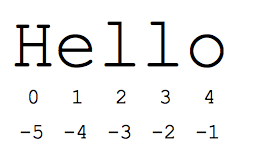
\includegraphics{hello_string.png}
		\caption{редни бројеви карактера у ниски}
		\label{slike:hello}
		\end{figure}
		Сад кад је познато како се може приступити појединим знаковима у ниски, могу се набројати које операције са нискама имамо. Постоји више операција са нискама. Табела која следи приказује операције са нискама:
		\begin{table}[h]
		\centering
		\begin{tabular}{|c|c|c|} \hline
		\multicolumn{3}{|c|}{\textbf{ОПЕРАЦИЈЕ СА НИСКАМА}}\\ \hline
		\textbf{Операције} & \textbf{Објашњење} & \textbf{Пример} \\ \hline
		+ & спајање ниски - конкатенација & s + t \\ \hline
		* & множење, одн. мултипликација ниски & s * 3 \\ \hline
		s[i] & враћа i-ти знак у ниски & s[-1] \\ \hline
		s[n:m] & враћа све знаке ниске између позиција n и m & s[2:4] \\ \hline
		len(s) & враћа целобројну дужину ниске & len("Hello!") \\ \hline
		str(n) & претвара број у ниску & str(23) \\ \hline
		\end{tabular}\medskip
		\caption{Операције са нискама}
		\label{tabele:strings}
		\end{table}
		
		Посебно је интересантна операција исецања ниске (енгл. \emph{slicе}), чиме се даје могућност да се од ниске исече и одвоји тачно онај део који је потребан.
		\begin{lstlisting}[caption = Комадање ниске, label = slice]
>>> s = "Hello"         # niska s pokazuje na niz slova Hello
>>> print (s[1:4])      # svi znakovi pocev od drugog zakljucno sa cetvrtim
ell
>>> print (s[1:])       # svi znakovi pocev od drugog do kraja niske
ello
>>> print (s[:])        # svi znakovi od pocetka do kraja
Hello
>>> print (s[1:100])    # svi znakovi pocev od drugog zakljucno sa stotim
ello                    # ako ne postoji 100-i znak, vraca se kraj niske
>>> print (s[-1])       # odredjuje se poslednji znak niske
o
>>> print (s[-4])       # odredjuje se 4. znak od pozadi
e
>>> print (s[:-3])      # svi znaci pocev od pocetka pa do treceg od pozadi
He
>>> print (s[-3:])      # svi znaci pocev od treceg od pozadi do kraja niske
llo		

\end{lstlisting}
		\subsubsection{Листе}
		Листа\index{Python!liste@листе} је мутабилна структура података, у којој се може сачувати секвенца произвољних елемената. Листу могу чинити бројеви, ниске или бројеви и ниске у једној листи. Листа може да садржи друге листе.\\
		 Листа се означава помоћу угластих заграда између којих се набрајају чланови листе, одвојени запетом. Ако између две угласте заграде нема ништа, креирана је празна листа. Листа се може мењати, могу се избацивати одговарајући чланови листе, може се променити садржај одговарајућих чланова, а листа се може и допунити новим члановима. Све ове особине чине листе врло корисним оруђем у програмирању.\\
		 
		 \begin{lstlisting}[caption = Креирање листе, label = lista]
>>> bitlsi = ['Pol', 'Dzordz', 'Ringo', 'Dzon']
>>> print(bitlsi)
['Pol', 'Dzordz', 'Ringo', 'Dzon']
		 \end{lstlisting}
		 \medskip
		 	 
		 \begin{lstlisting}[caption = Креирање празне листе, label = prazna_lista]
>>> prazna_lista = []
>>> print(prazna_lista)
[]
		 \end{lstlisting}
		 \medskip
		 
		 
		 		 Кад се креира листа под неким именом, онда то име (променљива) реферише на део меморије у који је уписана дата листа. \\
		 		 
		 \begin{figure}[here]
		 \centering
		 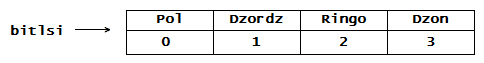
\includegraphics[scale = 0.50]{bitlsi1.png}
		 \caption{Креирање листе}
		 \label{slike:lista}
		 \end{figure}
		 Ако је потребно да се креира нова листа (на пример \emph{lista}) и њој додели вредност листе \emph{bitlsi}, тада ће и нова листа реферисати на исти меморијски простор. Ако изменимо садржај листе \emph{lista}, аутоматски се мења и садржај листе \emph{bitlsi}. 
		 \begin{figure}[here]
		 \centering
		 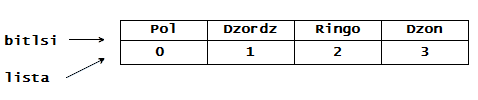
\includegraphics[scale=0.50]{bitlsi2.png}
		 \caption{lista = bitlsi }
		 \label{slike:kopiranje}
		 \end{figure}
		 На сликама \ref{slike:lista} и \ref{slike:kopiranje}, се може уочити редни број чланова листе формира на исти начин као и код ниски, дакле: први члан је под редним бројем 0, следећи је 1, итд. Ако је потребно обележити последњи члан листе, користи се редни број -1, претпоследњи је -2, итд. \\
		 На листе је могуће применити и исецање листи, на сличан начин како је описано при опису операција са нискама.\\
		 
		 
		 \begin{lstlisting}[caption = Исецање листи, label = list_slice][here]
>>> bitlsi = ['Pol', 'Dzordz', 'Ringo', 'Dzon']
>>> print (bitlsi[0:2])
['Pol', 'Dzordz']
>>> print (bitlsi[1])
Dzordz
>>> print (bitlsi[-1])
Dzon
		\end{lstlisting}
		\medskip\pagebreak
		Оно што највише разликује листе од ниски је способност мутације. Листама се могу додавати или избацивати чланови, листе се могу сортирати. У наредној табели набројане су операције са листама. \\
		\begin{table}[here]\index{Python!operacijesalistama@операције са листама}
		\centering
		\begin{tabular}{|c|c|c|}\hline
		\multicolumn{3}{|c|}{\textbf{ОПЕРАЦИЈЕ СА ЛИСТАМА}}\\ \hline
		\textbf{Операције} & \textbf{Објашњење} & \textbf{Пример} \\ \hline
		list[i] & враћа i-ти члан листе & bitlsi[0] \\ \hline
		list[m:n] & даје све чланове почев од m-тог па закључно са n-1 & bitlsi[0:2] \\ \hline
		len(list) & враћа број чланова листе & len(bitlsi) \\ \hline
		+ & спаја две листе & bitlsi + stonsi \\ \hline
		* & мултипликује садржај листе & bitlis * 2 \\ \hline
		\multicolumn{3}{|c|}{\textbf{МЕТОДЕ}}\\ \hline
		append & додаје нови члан листе на крај листе & bitlsi.append('Pete')\\ \hline
		insert & додаје нови члан на датом месту у листи & bitlsi.insert(1, 'Brian') \\ \hline
		index & враћа редни број датог члана & bitlsi.index('Pol') \\ \hline
		remove & брише дати члан листе & bitlsi.remove('Dzon') \\ \hline
		pop & враћа и брише последњи члан листе & bitlsi.pop() \\ \hline
		sort & сортира листу & bitlsi.sort() \\ \hline
		\end{tabular}
		\caption{Операције и методе са листама}
		\label{tabela:liste}
		\end{table}
		\begin{lstlisting}[caption= Мењање листе, label = mutacija_list][here]
>>> bitlsi = ['Pol', 'Dzordz', 'Ringo', 'Dzon']
>>> bitlsi.append('Pit')
>>> print(bitlsi)
['Pol', 'Dzordz', 'Ringo', 'Dzon', 'Pit']
>>> bitlsi.remove('Pit')
>>> print(bitlsi)
['Pol', 'Dzordz', 'Ringo', 'Dzon']
>>> bitlsi.insert(1, 'Pit')
>>> print(bitlsi)
['Pol', 'Pit', 'Dzordz', 'Ringo', 'Dzon']
>>> bitlsi.pop()
'Dzon'
>>> print(bitlsi)
['Pol', 'Pit', 'Dzordz', 'Ringo']
>>> bitlsi.sort()
>>> print(bitlsi)
['Dzordz', 'Pit', 'Pol', 'Ringo']
		\end{lstlisting}
		
		Листе су моћно средство програмирања у Python-у, али потребно је бити опрезан кад се употребљавају одговарајуће методе, како се не би јавила грешка(нпр. покушај да се избаци елемент који не постоји у датој листи, доводи до грешке). Такође, треба бити опрезан и код мутирања листе, јер као што је показано ако две променљиве реферишу на исту листу, мењање једне, проузрукује и мењање друге. 
		\subsubsection{Мапе}\label{subsec:maps}
		Мапе\index{Python!mape@мапе} или речници(енгл. \emph{dictionaries}) представљају колекцију елемената, слично као што је то случај и са листама. Разлика између мапа и листа је у томе што се код мапа уместо редних бројева чланова листа, користе парови кључева и њима одговарајућих вредности. Дакле, мапа је структура која се записује тако што се између витичастих заграда набрајају парови који чине један кључ и једна или више вредности везаних за тај кључ. Вредности могу бити бројеви, ниске, листе, уређене n-торке. 
		\begin{lstlisting}[caption = Разлика између листе и мапе, label = map_vs_list]
>>> bitl_list = [['Pol', 'bas', 'vokal'],
	         ['Dzordz', 'gitara'],
	         ['Ringo', 'bubanj'],
	         ['Dzon', 'gitara', 'vokal']]
>>> print (bitl_list)
[['Pol', 'bas', 'vokal'], ['Dzordz', 'gitara'], ['Ringo', 'bubanj'], 
['Dzon', 'gitara', 'vokal']]
>>> bitl_map = {'Pol' : ['bas', 'vokal'],
	        'Dzordz' : ['gitara'],
	        'Ringo' : ['bubanj'],
	        'Dzon' : ['gitara', 'vokal']}
>>> print(bitl_map)
{'Pol': ['bas', 'vokal'], 'Dzordz': ['gitara'], 
'Ringo': ['bubanj'], 'Dzon': ['gitara', 'vokal']}
		\end{lstlisting}
		Ако је потребно да се прикаже шта је Пол свирао, уколико су подаци о групи запамћени као листа, потребно је знати који је Пол редни број у листи, док код мапе редни број не постоји и вредностима се приступа помоћу кључа.
		\begin{lstlisting}[caption = Кључ и вредност, label = key_value]
>>> print (bitl_map['Pol'])
['bas', 'vokal']
		\end{lstlisting}
		Ако је задатак да се утврди ко је све свирао гитару у Битлсима, потребна је петља, тако да ће тај задатак бити решаван у поглављима која следе, када буду обрађивале петље и модули.\\
		Због природе мапа, мутација је прилично другачија у односу на листе. Да би се додао нови елемент, односно пар кључ-вредност, потребно је уз име мапе ставити нови кључ и доделити му вредност или изменити постојећу. Такође помоћу команде \emph{del}, могуће је обрисати кључ, а тиме и вредност везану за њега.
		\begin{lstlisting}[caption = Мутација мапа, label = mutacija_mapa]
>>> bitl_map['Pit']='bubanj' 
>>> bitl_map['Dzordz']=['gitara', 'vokal'] # dodan je vokal Dzordzu
>>> del bitl_map['Pit']
		\end{lstlisting}
		Могуће је креирати и празну мапу, једноставно се остави празан простор између две витичасте заграде.
		\begin{lstlisting}[caption = Креирање празне мапе, label=prazna_mapa]
>>> prazna_mapa = {}
		\end{lstlisting}
		Методи и функције за рад са мапама су различити у односу на листе, јер не постоје, на пример \emph{pop} и \emph{append} методе који омогућавају мутацију, већ да би се мењала мапа потребно је знати који елемент се убацује, мења или избацује из дате мапе.
		\begin{table}[here]
		\centering
		\begin{tabular}{|c|c|c|} \hline
		\multicolumn{3}{|c|}{\textbf{МЕТОДИ И ФУНКЦИЈЕ ЗА РАД СА МАПАМА}} \\ \hline
		\textbf{Метода} & \textbf{Објашњење} & \textbf{Пример} \\ \hline
		map[key]=value & Додељивање или мењање вредности кључа & bitlsi['Dzon'] = 'vokal' \\ \hline
		del map[kljuc] & Брисање кључа и вредности из мапе & del bitlsi['Pol'] \\ \hline
		keys() & Метод којим се сви кључеви дате мапе враћају као листа & bitlsi.keys() \\ \hline
		values() & Метод којим се све вредности дате мапе враћају као листа & bitlsi.values() \\ \hline
		items() & Метод који враћа листу уређених парова кључ, вредност & bitlsi.items() \\ \hline
		\end{tabular}
		\caption{Методе и функције за рад са мапама}
		\label{tabela:mape}
		\end{table}
		\subsubsection{Уређене n-торке}
		У Python-у постоји начин да подаци сместе у уређене n-торке\index{Python!tapl@тапл}, где $n \in \mathbb{N}\cup\{0\}$. Подаци се смештају између две заграде и раздвојени су зарезом. Python интерпретатору није потребно да их ставимо између заграда, док год су подаци раздвојени зарезом, већ ће он свако набрајање схватити као уређену n-торку, чак и ако нема заграде. 
		\begin{lstlisting} [caption = Креирање уређене n-торке, label = tuple]
>>> fibo = (0, 1, 1, 2, 3)
>>> print (fibo)
(0, 1, 1, 2, 3)

>>> fibo1 =0, 1, 1, 2, 3  # uredjena n-torka bez zagrada
>>> print (fibo1)
(0, 1, 1, 2, 3)		  
		
>>> prazan = () # kreiranje prazne uredjene n-torke
>>> print (prazan)
()

>>> jedan_clan = (1,) # jednoclana uredjena n-torka mora imati
>>> print (jedan_clan) # zarez, iako ne postoji drugi broj
(1,)
		\end{lstlisting}
		\pagebreak
		У уређеним n-торкама је могуће сместити вредности и других типова података, као што су бројеви и ниске. Такође, могуће је сместити и листе и друге уређене n-торке, док год се поштује горе наведена синтакса. 
		\begin{lstlisting}[caption = Уређене n-торке могу садржати и ниске и  листе и друге уређене n-торке, label = str_lst_tuple]
>>> niska = ('a', 'b')
>>> print (niska)
('a', 'b')
>>> lst = ([1, 2, 3], [1,2])
>>> print (lst)
([1, 2, 3], [1, 2])
>>> tapl = ((1,), (), (1, 2, 3))
>>> print (tapl)
((1,), (), (1, 2, 3))
		\end{lstlisting}
		Оно што највише разликује уређене n-торке од осталих типова података је да су они у потпуности непроменљиви. Када се креира уређена n-торка, могуће је искључиво користити њене вредности, док је немогуће мењати или додавати вредности уређених n-торки. Могуће је, уколико се за тим укаже потреба доћи  до појединих чланова уређених n-торки, ако се зна њихов редни број, а могуће је исецати уређене n-торке, слично као код ниски. 
		\subsection{Услов}
		У програмирању се често постављају "да" или "не" питања и доносе се одлуке шта урадити у односу на одговор. На пример, може се поставити питање: "Да ли студирате математику мање од 10 година?" и ако је одговор "Да", то се може протумачити као: "Ви сте сјајан студент!".\\
		Често се комбинују услови(питања) и одговори у оквиру \emph{if}\index{Python!if@\emph{if}} наредбе. Услова може бити више у једном изразу и можемо их комбиновати. 
		
		\subsubsection{Програмски блок}
		Линије кода после двотачке морају бити постављене у блок, иначе их Python интерпретатор неће правилно протумачити. Да би блок био разумљив интерпретатору, блок мора бити увучен тачно четири (празна) карактера\footnote{Празни карактери се на енглеском називају белине(енгл. \emph{Whitespaces}}  у односу на линију која је захтевала програмски блок\cite{PEP}.\\
		Линије кода се групишу у исти блок морају бити на истој удаљености од маргине\footnote{\emph{indent}, \emph{енгл.}}. Структура блокова у Python-у би могла да буде оваква:\\
		\begin{figure}[here]
		\centering
		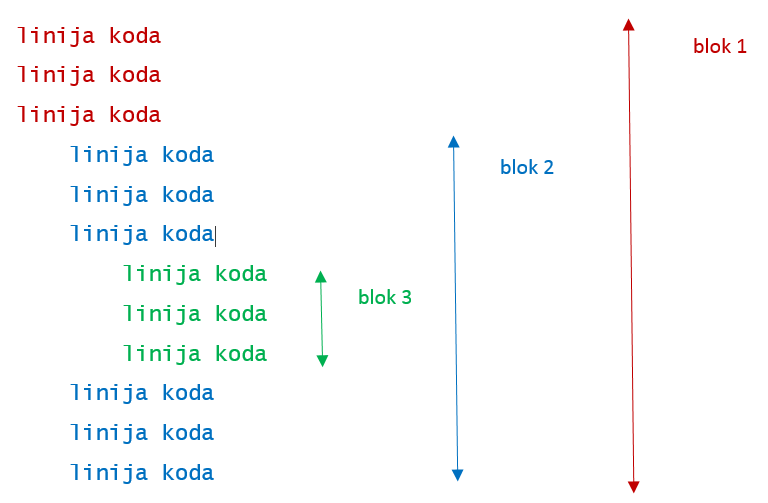
\includegraphics[scale=0.5]{whitespace.png}
		\caption{Пример програмских блокова у Python-у}
		\label{slike:whitespace}
		\end{figure}
		
		\subsubsection{Наредба if}
		Следи начин на који би се претходно питање, тј. услов, могао реализовати:
		\begin{lstlisting}[caption = Пример услова, label = if]
>>> godine_studiranja = 6
>>> if godine_studiranja < 10:
        print('Vi ste sjajan student') 
		\end{lstlisting}
		\subsubsection{Наредба if-then-else}
		
		Могуће је проширити дефиницију \emph{if} наредбе како би, на пример у претдном примеру пронашло колико је ко година студирао. За такву структуру је потребна кључна реч \emph{else}\index{Python!else@\emph{else}}. \\
		Укратко, ако је услов у \emph{if} делу тачан, извршава се блок испод те линије, а ако није тачан, извршава се блок испод \emph{else} линије ако та линија кода постоји. Ако не постоји, а услов није тачан, неће се ништа извршити, већ интепретатор наставља извршавање даљих линија к\^{о}да. 
		\begin{lstlisting}[caption = Пример за наредбе IF - ELSE, label = ifelse]
>>> if godine_studiranja < 10:
        print('Vi ste sjajan student')
    else:
        print('Nije strasno')
        \end{lstlisting}
        \subsubsection{Услови и комбиновање услова}
        Упоређивање две величине даје једну од две вредности: тачно или нетачно. Следећи оператори се користе за упоређивање:
        \begin{table}[here]
        \centering    
        \begin{tabular}{|c|c|} \hline
        \textbf{Оператор} & \textbf{Дефиниција} \\ \hline \hline
        == & једнако \\ \hline
        != & није једнако \\ \hline
        > & веће од  \\ \hline
        < & мање од \\ \hline
        >= & није мање од \\ \hline
        <= & није веће од \\ \hline
        \end{tabular}\medskip
        \caption{Оператори упоређивања}
        \label{tabele:opporedjenja}
        \end{table}\\
        
        На пример, ако је потребно проверити да ли нека особа има 20 година, користи се оператор једнакости: \emph{if godine==20:}\\
        
        Услови се комбинују коришћењем логичких оператора \emph{и} и \emph{или}. Оператор конјункције је \emph{and}, а дисјункције \emph{or}. Тако да на пример можемо овако рећи: \emph{if godine > 18 and bodovi >=50:} и слично.
        \pagebreak
        Такође, у услову се може испититати да ли је или није неки елемент члан листе, уређене n-торке, ниске или мапе.  За то се користе оператори \emph{in} и \emph{not in}. На пример: \emph{if elem not in lista:}. 
		\subsection{Петље}
		Програмери не воле много да се понављају, штавише у Python-овом "правилнику" за писање к\^{о}да, PEP\cite{PEP}\index{PEP}, постоји правило \emph{DRY}, односно \textbf{Don't Repeat Yourself}\footnote{енгл., \emph{не понављај се}}, но понекад је потребно да интерпретатор одређени блок поновљено извршава коначно много пута. Такав део програма се назива петља. Постоји више врста петљи у Python-у, овде ће бити описане две. 
		\subsubsection{Петља while}
		Као што дословни превод са енглеског каже, \emph{док}\index{Python!while@\emph{while}} је одређени услов испуњен, исти кодни блок се врти у петљи. Ако услов није тачан, петља се прекида и извршавање програма се наставља иза петље. Услови петље се дефинишу на претходно описани начин. На пример:
		\begin{lstlisting}[caption = Пример while петље, label = while]
>>>i=1
>>>while i<=10:
       print(i)
       i=i+1
		\end{lstlisting}
		Ако је потребно да се изађе из петље пре него што услов постане нетачан, користи се кључна реч \emph{break}. У том случају петља се прекида и програм наставља даље да се извршава од прве наредбе која следи иза петље. 
		\pagebreak
		\subsubsection{Петља for}
		Ова\index{Python!for@\emph{for}} петља се користи на сличан начин као и петља \emph{while}, с тиме да се користи нова кључна реч - \emph{range}. На пример:
		\begin{lstlisting}[caption = Примери \emph{for} петље, label = for]
>>>for i in range(1, 11):
      print(i) // stampaju se brojevi od 1 do 10
>>>for i in list:
      print(list[i]) //stampaju se elementi liste
		\end{lstlisting}
		И \emph{for} и \emph{while} петље се могу угњежђавати и то вишеструко са више петљи. 
		\subsection{Функције и модули}
		Ако се довољно често употребљава одређени кодни блок, који би могао поново да се искористи, онда је пожељно правити функцију. Организација к\^{о}да у којој се крупне целине деле на мање и смештају у функције је пожељна, јер омогућава бољу прегледност к\^{о}да, а тиме и лакше проналажење грешака. Такође, у том случају је могуће лакше да мењати к\^{о}д, прилагођавати га другим апликацијама, итд.
		\subsubsection{Функције у Python-у}
		Да би се употребила функција \emph{func}\index{Python!funkcije@функције}, која има улазне параметре, на пример $a_{1}, a_{2},\dots, a_{n}$, она мора да се позове у к\^{о}ду са:
		\begin{lstlisting}
>>>func(a1, a2, ..., an)
		\end{lstlisting}  
		Дефинисање функције почиње са кључном речи $def$\index{Python!def@\emph{def}}, иза које се наводи назив и параметри функције. Функција не мора имати параметре, а ако их има, онда их има коначно много. На крају реда се поставља специјални знак - двотачка, која у Python-у има улогу да упозори интерпретатор да иза ње следи кодни блок. У следећи ред к\^{о}да, увученом за 4 празна карактера, започиње кодни блок дате функције. 
		\begin{lstlisting}[caption = Дефинисање функције, label = func]
>>>def min(a, b):
      if a < b:
          return a
      else:
          return b
		\end{lstlisting}
		Да би функција вратила неку вредност потребно је да у дефиницији функције постоји кључна реч $return$\index{Python!return@\emph{return}} после које се наводи вредност која ће бити резултат функције. 
		\subsubsection{Модули}
		Модули\index{Python!modul@модули} служе за груписање функција, променљивих и других структура у веће и моћније програме. Неки модули су уграђени у сам Python: на пример, $tkinter$\footnote{$tkinter$ служи за прављење игара у Python-у}. Такође, постоји могућност учитавања модула које су други поставили на интернет, а који помажу лакшем и бржем писању жељеног к\^{о}да. Неки од познатијих таквих модула су $PIL$\footnote{PIL више није актуелан од верзије Pythona 2.6. Наследник овог модула је $PILLOW$}  (Python Imaging Library), Panda3D, итд.\\
		 Да би се користио модул, потребно је на почетку програма употребити кључну реч $import$, после које се наводи име модула. На пример: $import$ \emph{time}.
		\subsection{Класе и објекти}
		Модеран програмски језик не може се замислити без подршке објектно-ориијентисаном програмирању\footnote{краће \emph{ООП}}. Python, наравно, омогућава коришћење објектно-оријентисаног програмирања и даје му пуну подршку.  
		\subsubsection{Објектно-оријентисано програмирање}
		Овај рад нема амбицију да се бави Објектно-оријентисаним програмињем(у даљем тексту: ООП). У даљем тексту ће се у краћим цртама навести значај, особине и предности ООП. \\
	Појам Објектно-оријентисаног програмирања први пут се помиње почетком '70-их година прошлог века, приликом представљања програмског језика $Smalltalk$ (први језик који је у себи имао елементе ООП је био $Simula67$). Касније се највише везује за програмски језик Java\index{Python!Java@\emph{Java}}, да би се данас широко примењивао у програмирању. \\
	     Објектно-оријентисано програмирање је засновано на концепту објекта. \emph{Објекти} су структуре података са придруженим скупом процедура и функција које се називају \emph{методи} и служе за рад са подацима који припадају објекту. Уобичајено је да су методи једини начин за рад са објектима. Сваки објекат је примерак или инстанца неке \emph{класе}. У класи се дефинише садржај објеката те класе и скуп метода који ће омогућити рад са објектима.\\
	     Готово у свим објектно-оријентисаним програмским језицима постоји \emph{наслеђивање} као механизам за креирање нових класа из већ постојећих. На тај начин се добијају наткласе и поткласе. 
		 Уобичајена је могућност у објектно-оријентисаном програмирању дефинисање и поткласа класе, која је у односу на своју супер-класу \emph{дете}, док је супер-класа \emph{родитељ}. Поткласа наслеђује све садржаје објеката класе и методе од наткласе. Типичан пример за овакав начин наслеђивања је класа Животиња, где можемо дефинисати поткласе Сисари, Инсекти, Птице, Рибе, итд. Такође, можемо дефинисати и класу Торбари, која ће бити поткласа Сисара и тај процес наслеђивања можемо продужити коначно много. 
		\subsubsection{Класе и објекти у Python-у}
		Да би се креирала класа у Python-у, потребно је користити кључну реч $class$, после које се наводи име класе и евентуално класу наткласе, које је та класа наследила. На пример:
		\begin{lstlisting}[caption=Дефинисање класа, label=class]
>>>class Zivotinje:
      pass
>>>class Sisari(Zivotinje):
      pass
		\end{lstlisting}
	    Кључна реч $pass$\index{Python!pass@\emph{pass}} значи да та класа не садржи никакве особине објеката нити методе.\\
\pagebreak	    
	    Када постоји потреба за увођењем конкретног примерка класе, тј. објекта\index{Python!objekti@објекти} неке класе, тада је потребно само да навести име објекта и после знака једнакости навести класу и особине које припадају датом објекту, као у следећем примеру: 
	    \begin{lstlisting}[caption=Креирање објекта, label=objects]
>>>class Macke(Sisari):
      pass
>>>tosa = Macke()	    
	    \end{lstlisting}
	    У Python-у не постоје конструктори и деструктори као у неким другим објектно-оријентисаним програмским језицима. Довољно је навести име класе и инстанца је препозната код интерпретатора. 
		\subsubsection{Методи}
		У класи је могуће креирати скуп функција\index{Python!metodi@методи}. Такве функције се називају методима дате класе. Креирање метода се врши дефинисањем функције унутар класе.\\
		Објекту се додељује метод, тако што се после имена објекта поставља тачка и наводи име метода са аргументима, набројаним унутар заграде. Метод не мора да има аргументе. 
		\begin{lstlisting}[caption= Методи класе, label=method]
>>>class Macke(Sisari):
       def predenje():
           print('purrrrr')
>>>tosa.predenje()
>>>purrrrr 
		\end{lstlisting} 
		
		 \pagebreak 
		 

		
\section{Претрага Интернета и обрада хипервеза}
\subsection{Проналажење информација}
Проналажење информација\index{pronalazenje informacija@проналажење информација} може се дефинисати као процес претраживања унутар неког документа и/или колекције докумената за потребном информацијом.\cite{langville2011google}. Кроз историју се проблем проналажења информација у документима почео решавати још у 5. веку п.н.е. у Античкој Грчкој, кад је први пут уведен \emph{садржај} у неки од свитака папируса, пошто књиге у данашњем облику тада још нису постојале. У Старом Риму проблем су решавали етикетама налик на данашње \emph{Post-it} налепнице. Све се, наравно, променило са проналаском штампарске машине, средином 15. века. Крајем 19.века почиње да се имплементира Дјуијев\index{Djui@Дјуи} децимални систем\footnote{Dewey, 1872. Сортирао је колекције према тематици, на пример, троцифреним бројевима који почињу са 1 је означавао филозофију, са 2 религију, итд. Тако да је, на пример, књига са идентификационим бројем 142 означавала књигу о филозофији.} , каталог картица. У 20. веку долази до употребе технологије у претраживању докумената, па се тако појављују микрофилмови. У '60-им годинама прошлог века направљена је прва машина која је радила претрагу информација, а ради се о \emph{MARC}\footnote{енгл., \emph{Machine Reading Catalog}}\index{MARC@\emph{MARC}} рачунару. Данас се у традиционалном претраживању\index{tradicionalno pretrazivanje@традиционално претраживање} и проналажењу информација користи систем картица (на пример у библиотекама), али и компјутерски помогнути системи. У овим последњим постоје три карактеристична модела за претраживање: \emph{буловски}, \emph{векторски}, \emph{модели вероватноће}\cite[Ch 1.2]{langville2011google}. Постоји на хиљаде модела, али су сви настали као варијанте три горе наведена.\\
\textbf{Буловски модел}\index{tradicionalno pretrazivanje@традиционално претраживање!Bulovski model@Буловски модел} користи систем егзактног подударања да нађе документ који корисник захтева. Име је добио по Буловој алгебри, чије логичке операторе користи. Не постоји концепт парцијалног подударања што је велики проблем, ако је потребно да пронаћи документ, за који се не зна тачан назив. Проблеми претраживања информација, као што су проблем синонима и проблем вишезначности, овде се не могу избећи. \\
\textbf{Векторски модел}\index{tradicionalno pretrazivanje@традиционално претраживање!Vektorski model@Векторски модел} је увео Џералд Салтон,'60-их година прошлог века. Базира се на трансформацији текстуалних података у нумеричке векторе и матрице и примењује се матрична анализа за откривање повезаности кључних речи. Овакви модели решавају проблеме синонима и вишезначности. Резултати се могу презентовати сортирани према степену релевантности.\cite{berry2005understanding}\\
\textbf{Модели вероватноће}\index{tradicionalno pretrazivanje@традиционално претраживање!Modeli verovatnoce@Модели вероватноће} покушавају да процене вероватноћу којом ће корисник наћи жељени документ у односу на упит. Резултати се могу поређати по изгледима релевантности. Није једноставно имплементирати овакве моделе у рачунарско окружење. \\
\subsection{Проналажење информација на вебу}
Када је у марту 1989. године британски инжењер Тим Бернерс-Ли\index{Tim Berners Lee} послао предлог\footnote{\texttt{http://www.w3.org/History/1989/proposal.html}}  да се унапреди информациони систем у \emph{CERN}-у\footnote{Европска организација за нуклеарна истраживања (франц., \emph{Conseil Européen pour la Recherche Nucléaire})}\index{CERN@\emph{CERN}}, није ни слутио у шта ће се претворити једноставна потреба за хипервезивањем основних података о запосленим у \emph{CERN}-овом информационом систему\cite{berners2004weaving}. Тим Бернерс-Ли је за потребе новог информационог система измислио нови језик који је назвао \emph{Hypertext Markup Language}\index{HTML@\emph{HTML}}, одн. \textbf{HTML}. Такође, осмислио је и читач HTML, к\^{о}да који је назвао \emph{World Wide Web} и он се у исто време користио и за прављење веб страница. \index{WWW@\emph{WWW}}\\
Од прве веб странице из маја 1990. године до данас је прошло више од 20 година, а у овом тренутку постоји неколико милијарди веб страница. Јасна је мотивација која се од почетка јавила корисницима веба, а то је како наћи праву информацију. Веб\index{veb@веб} је огроман, динамичан, самоорганизован и хиперповезан.\cite[Ch 1.3.1]{langville2011google} Свако може поставити веб страницу\index{veb@веб!veb stranice@веб странице}. Странице се мењају дневно, па чак и чешће. Нове странице се појављују сваки минут. То су реални проблеми веб претраживања, на које није могло да одговоро традиционално претраживање информација. Такође, корисници ретко погледају више од 10 до 20 докумената који су понуђени, што појачава потребу да резултати морају бити јако прецизни и брзо достављени кориснику.\\
Први Интернет претраживач је био \emph{Archie}\index{Archie@\emph{Archie}}, направљен 1990. године, од стране канадског студента Алана Емтејџа. Примарни протокол је био \emph{ftp}. Први робот\index{robot@робот} који је аутоматски индексирао странице звао се \emph{World Wide Web Wanderer} који је своје резултате стављао у прву базу хипервеза веб страница \emph{Wandex}\index{robot@робот!Wandex@\emph{Wandex}}. До средине '90-их направљено је на хиљаде \emph{веб-паукова} тј. робота који су складиштили информације на вебу. На жалост, нису знали како да искористе те информације на добар начин. 1994. године појавио се \emph{Yahoo}\index{veb pretrazivac@веб претраживач!Yahoo@\emph{Yahoo}} као збир неколико популарних страница и са директоријумом популарних страница. У том тренутку \emph{Yahoo} се не може сматрати претраживачем. Али 1994. године се појављују два значајна \emph{веб-паука}\index{crawler@\emph{crawler}}-а, \emph{WebCrawler}\index{crawler@\emph{crawler}!WebCrawler@\emph{WebCrawler}} и \emph{Lycos}\index{crawler@\emph{crawler}!Lycos@\emph{Lycos}}, чији се број сакупљених хипервеза мерио у десетинама милиона. У децембру 1995. године појављује се први прави веб претраживач\index{veb pretrazivac@веб претраживач} \emph{AltaVista}\index{veb pretrazivac@веб претраживач!AltaVista@\emph{AltaVista}} који је омогућавао примену логичких оператора. \emph{AltaVista} је имала врло лош алгоритам рангирања страница, који се заснивао на провери тзв. мета-података из заглавља HTML документа и врло лако је могао да се злоупотреби и зато је пројекат пропао крајем 20. века, а са појавом \emph{Google}-а\index{veb pretrazivac@веб претраживач!Google@\emph{Google}}. Два су кључна алгоритма за даљи развој веб претраживања: \emph{PageRank}\index{PageRank@\emph{PageRank}} и \emph{HITS}\index{HITS@\emph{HITS}}. Први је омогућио Гуглу да постане оно што данас јесте, а то је најкоришћенији претраживач са највише индексираних страница, док је \emph{HITS} дело Џона Клајнберга из IBM-а купљен од стране \emph{Тeome}, данашњег \texttt{ask.com}. Оба алгоритма су се јавила независно један од другог исте, 1998. године. Више о PageRank алгоритму у даљем делу рада. Данас имамо много интернет претраживача, попут Google-а\index{veb pretrazivac@веб претраживач!Google@\emph{Google}}, Bing-а\index{veb pretrazivac@веб претраживач!Bing@\emph{Bing}}, Yahoo-а\index{veb pretrazivac@веб претраживач!Yahoo@\emph{Yahoo}}, итд. \\
\subsection{Процес веб претраживања}\label{subsec:web}

Веб претраживач\index{veb pretrazivac@веб претраживач} је веб апликација која ће претражити веб странице, извући све могуће хиперлинкове, рангирати их и на крају дати најбоље могуће решење за задату кључну реч. Апликација се састоји из више елемената:
\begin{itemize}
\item модул веб-паука
\item модул индексизације
\item индекс
      \begin{itemize}
      \item индекс садржаја
      \item индекс структуре
      \item индекс за специјалне сврхе 
      \end{itemize}
\item складиште страница
\item модул упита
\item модул рангирања

\end{itemize}

Процес се састоји од узајамног деловања претходно набројаних модула. Тако веб-паук скупља странице по вебу, целе странице одлаже у \emph{складиште веб страница}, док хипервезе шаље у индекс, који их поставља уз кључне речи које добија из модула индексовања. Кад корисник пошаље упит, модул упита тражи од индекса скуп свих решења, која се кроз модул рангирања на крају постављају као резултати корисниковог упита. Модел процеса може се представити као што је то урађено на слици  \ref{slike:crawling}.
\begin{figure}
\centering
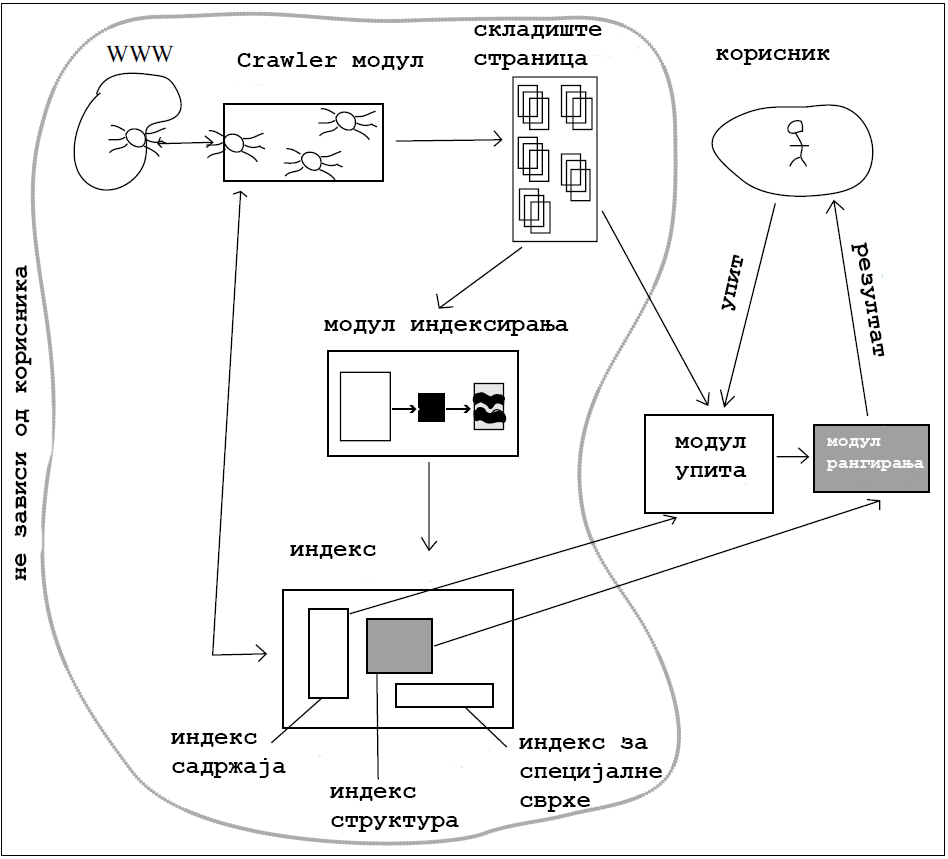
\includegraphics[scale=0.5]{crawling.png}
\caption{Процес веб претраживања \cite[Ch 1.3.2]{langville2011google}}
\label{slike:crawling}
\end{figure}

	\subsection{Извлачење хипервезе}
	У процесу реализације к\^{о}да веб претраживача, прво је потребно написати програм веб-паука, који ће претражити страницу и наћи прво један, па онда и све остале хипервезе. Да би се пронашла хипервеза, потребно је знати како изгледа веб страница.
		\subsubsection{Структура HTML странице}
		Веб страница\index{HTML@\emph{HTML}}\index{veb@веб!veb stranice@веб странице} је заправо само дугачак низ карактера образованих у HTML к\^{о}д. Веб прегледач претвара к\^{о}д у изглед који се обично добија на екрану приликом избора неке странице. Да би се видео дати к\^{о}д који генерише веб страницу,  зависно од веб прегледача који се користи (\emph{Internet Explorer}, \emph{Firefox}, \emph{Safari} или \emph{Chrome}, на пример), потребно је потражити опцију "View Page Source", "View Source" или слично. 
		Структура овог рада не омогућава претерано улажење у HTML\index{HTML@\emph{HTML}}, те ће се упрошћено навести како изгледа структура HTML к\^{о}ода\footnote{више о томе на следећој страници \texttt{http://www.w3.org/TR/html401/struct/global.html}}. На пример:
		\begin{itemize}
		\item <html> таг;
		\item Заглавље, у којем се налазе подаци о наслову странице, аутору, разним  мета подацима везаним за страницу и све то се налази између <head> и </head> ознака;
		\item Садржај странице, који се исписује између <body> ознака;
		\item затвара се </html> ознаком
		\end{itemize}
		Интересантно за овај рад је како су означене хипервезе у том к\^{o}ду.
		\subsubsection{HTML <a> tag}
		За веб-паука од највеће важности је пронаћи хипервезе ка другим  веб страницама. Хипервезе у HTML\index{HTML@\emph{HTML}!a@<a>} к\^{о}ду се налазе унутар <а> ознаке. Наиме, хипервеза се задаје на следећи начин:
		\begin{lstlisting}[caption = <a> ознака, label = a_tag]
		<a href="<url>">
		<a href="http://www.matf.bg.ac.rs">
		\end{lstlisting}
		Дакле, да би се пронашла хипервеза унутар HTML к\^{о}да, потребно је прво пронаћи <a> ознака.
		\subsubsection{Налажење првог хиперлинка}
		Алгоритам за налажење прве хипервезе\index{HTML@\emph{HTML}!hiperlink@хиперлинк} у HTML к\^{о}ду, почиње од налажења <a href=" дела, а сама хипервеза ће се наћи између знакова навода који следе после горе поменуто дела к\^{о}да. Следи к\^{о}д који то успешно ради:
		\begin{lstlisting}[caption = Налажење првог хиперлинка, label = {lst:first_url}, numbers = left]
# u promenljivoj page je smestena niska celog 
# HTML koda internet stranice
page = '<sadrzaj veb stranice>'  

# trazi se prvo pojavljivanje <a> oznake i 
# smesta se u promenljivu start_link
start_link = page.find('<a href=') 
		
# trazi se prvo pojavljivanje znaka navoda
start_quote = page.find('"', start_link) 
# trazi se zatvaranje navodnika
end_quote = page.find('"', start_link+1) 
# hiperveza je sve izmedju dva znaka navoda
url = page[start_quote + 1 : end_quote]
		\end{lstlisting}
	\subsection{Налажење свих хипервеза на страници}
	У претходном поглављу је дат к\^{о}д за налажење једне хипервезе\index{HTML@\emph{HTML}!hiperlink@хиперлинк} унутар HTML к\^{о}да. Да би се пронашле и остале хипервезе потребно је да наставити са процесом тражења следеће хипервезе. Ради тога, уводи се процедура која ће омогућити налажење следеће хипервезе. 
		\subsubsection{Процедура "get\_next\_target"}
		Да би се пронашла прва следећа хипервеза, односно да би се установило где ће бити почетак следеће хипервезе, потребно је пронаћи следећу <а> ознаку и тада поновити к\^{о}д за налажење прве хипервезе. Та процедура би требало да изгледа овако:
		
	\begin{lstlisting}[caption= Процедура налажења прве следеће хипервезе, label={lst:get_next_target_1}, numbers = left]
def get_next_target (page):
    start_link = page.find('<a href=')
    start_quote = page.find('"', start_link)
    end_quote = page.find('"', start_quote+1)
    url = page[start_quote+1:end_quote]
    return url, end_quote
	\end{lstlisting}
	Oвa процедурa враћa вредност хипервезе коју је пронашла, али и позицију завршног знака навода, како би се знало где је стала процедура и наставило са тражењем осталих хипервеза.
		\subsubsection{Ако нема линкова?}
		Потребно је решити проблем са горе поменутом процедуром у ситуацији да нема хипервеза у страници. Решење је да се постави услов, ако се не нађе почетак хипервезе, онда се враћа кључна реч \lstinline{None}, која означава празну ниску. 
		\begin{lstlisting}[caption = Испитивање да ли страница садржи хипервезу, label={lst:get_next_target_2}, numbers = left]
def get_next_target (page):
    start_link = page.find('<a href=')
    if start_link == -1:
        return None, 0
    start_quote = page.find('"', start_link)
    end_quote = page.find('"', start_quote+1)
    url = page[start_quote+1:end_quote]
    return url, end_quote
		\end{lstlisting}
		За испитивање у услову је коришћена вредност -1, јер Python враћа ту вредност ако не нађе задату ниску, тј. ако ниска не постоји.
		\subsubsection{Све хипервезе}
		Сад је могуће, користећи процедуру get\_next\_target(в. к\^{о}д \ref{lst:get_next_target_2}), одштампати све хипервезе\index{HTML@\emph{HTML}!hiperlink@хиперлинк} једне веб странице. Претпоставља се да је у променљивој \emph{page}, смештен HTML к\^{о}д неке веб странице.
		\begin{lstlisting}[caption=Процедура штампања свих хипервеза, label={lst:print_all_links}, numbers = left	]
def print_all_pages(page):
    while True:
         url, endpos = get_next_target(page)
         if url:
             print url
             page = page[endpos:]
         else:
             break
		\end{lstlisting}
        У претходном коду користи се "while True", пошто је потребно налазити нове хипервезе све док их има на страници, а ако их нема, наредбом \lstinline{break} излази се из петље.
    \section{Креирање "веб-паука"}    
	\subsection{Смештање хипервеза у листу}
	Користећи претходно описано проналажење свих хипервеза(в. к\^{о}д \ref{lst:print_all_links}), а за потребе креирања веб-паука, потребно је сакупити све хипервезе у неку колекцију, како би касније ти подаци могли бити даље процесуирани. \\
	
		У наредном к\^{о}ду, све хипервезе ће бити скупљене у листу. Уместо листе, могуће је користити и друге структуре као на пример мапе, али такви примери ће бити реализовани касније у оквиру овог рада.  
		\begin{lstlisting}[caption=Процедура смештања свих хиперлинкова у листу, label={lst:getalllinks}, numbers=left]
def get_all_links(page):
    links = []
    while True:
        url, endpos = get_next_target(page)
        if url:
            links.append(url)
            page=page[endpos:]
        else:
            break
    return links
		\end{lstlisting}
		У линији 4 се користе уређене n-торке, додељују се вредности променљивима \textbf{url} и \textbf{endpos}. Ако хипервеза постоји, биће додата у листу и траже се друге хипервезе почев од последњег знака наводника претходне хипервезе. Иначе, ако линк не постоји, петља се прекида и процедура враћа листу свих хипервеза\index{HTML@\emph{HTML}!hiperlink@хиперлинк} са дате веб странице.
	\subsection{Завршетак веб-паука}
	Веб паук би требао да нађе све хипервезе на задатој веб страници и да их смести у листу. Даље, веб-паук наставља процес следећи пронађене хипервезе и на тим веб страницама ће налазити нове хипервезе. Да се процес тражења хипервеза не би више пута понављао на истим веб страницама потребно је користити две променљиве:
	\begin{description}
	\item[tocrawl] у овој листи ће бити смештене странице које је потребно прегледати 
	\item[crawled] у овој листи ће бити смештене странице које су већ прегледане
	\end{description}
		\subsubsection{Завршни к\^oд}
		Претпоставља се да су познате процедуре \textbf{get\_next\_target} и \textbf{get\_all\_pages}, чији к\^{о}д је наведен у претходним поглављима(в. к\^{о}дове \ref{lst:get_next_target_2}, \ref{lst:get_all_pages}). Да би се к\^{о}д нове процедуре \textbf{crawl\_web} учинио прегледнијим, биће уведена и процедура \textbf{union} која прави унију две листе. Процедура \textbf{get\_page}  узима хипервезу и враћа HTML к\^{о}д те стране. Ако се страница не може отворити из разних разлога и/или је дата веб страница празна, процедура враћа празну ниску.  
		\begin{lstlisting}[caption=Веб паук, label={lst:crawlweb1}, numbers=left]
def get_page(url):
    try:
        import urllib
        return urllib.urlopen(url).read()
    except:
        return ""
     
def union(a, b):
    for e in b:
        if e not in p:
            p.append(e)

def crawl_web(seed):
    tocrawl = [seed]
    crawled = []
    while tocrawl:
        page = tocrawl.pop()
        if page not in crawled:
            union(tocrawl, get_all_links(get_page(page)))
            crawled.append(page)
    return crawled
		\end{lstlisting}
		Процедура прво поставља две листе, оно што је потребно претражити и ту поставља први елемент, иницијалну страницу. Друга променљива је она у коју се смештају странице које су већ претражене и она је иницијално празна. Кад се страница претражи, она се додаје у \textbf{crawled} листу да се не би више пута непотребно претраживала.\\
		  У линији 9 почиње петља, која ради док листа \textbf{tocrawl} има елемената. Кад листа више нема страница за скенирање, процедура враћа листу прегледаних страна. У петљи се скида последња хипервеза из \textbf{tocrawl} листе и на основу одговора после питања из услова да ли је та страница већ претражена, процедура је даље претражује или не. На крају хипервеза бива додата листи већ претражених страна. 
		\subsubsection{Ограничен број страна по свакој хипервези}
		Уколико не постоји потреба за претраживањем свих веб страница на које упућују хипервезе које су прегледане у току процесу тражења свих хипервеза који је описан у претходном поглављу , већ је потребно прегледати само првих неколико страница, тада да је могуће одредити колико ће се веб страница претражити. У наредном примеру, вредност максималног броја прегледаних страница ће бити смештена у променљиву \textbf{max\_pages}:
		\begin{lstlisting}[caption=Претраживање са ограниченим бројем страна, label={lst:crawlweb2}, numbers=left]
def crawl_web(seed, max_pages):
    tocrawl = [seed]
    crawled =[]
    count = 0 # vrednost brojaca inicijalno na 0
    while tocrawl and count < max_pages:
        page = tocrawl.pop()
        if page not in crawled:
            union(tocrawl, get_all_links(get_page(page)))
            crawled.append(page)
            count = count + 1 # iteracija brojaca posle svakog linka
    return crawled
		\end{lstlisting}
		Дакле, петљa se прекида ако је листа празна или ако је прекорачен максимални број хипервеза по страници. 
		\subsubsection{Ограничена "дубина" претраживања}
		Ефикаснији начин ограничавања рада веб-паука да не претражује све странице је да се постави одговарајућа "дубина" претраживања. Дубина ће у наредном примеру бити одређена променљивом \textbf{max\_depth}.
		\begin{lstlisting}[caption=Скенирање ограничено по дубини, label={lst:crawlweb3}, numbers=left]
def crawl_web (seed, max_depth):
    tocrawl = [seed, 0] # postavlja se 0 kao pocetna dubina
    crawled = []
    while tocrawl:
        layer = tocrawl.pop()
        depth = layer[1]
        if depth <= max_depth:
            for url in layer[0]:
                if url not in crawled:
                    union(tocrawl, [get_all_links(get_page(url)),depth+1])
                    # dubina se povecala za 1
                    crawled.append(url)
    return crawled
		\end{lstlisting}
		За потребе оваквог ограничавања, измењена је листа \textbf{tocrawl}, у којој сада постоји пар елемената: страница и број. Број се повећава кад се прегледају све хипервезе са одређене странице и пређе на нову страну. Тако се  ограничава веб-паук да после одређеног броја прегледаних страница заустави свој рад.
		\pagebreak
	\section{Добијање одговора на задати упит}	
	\subsection{Одговори на упите}
	Претраживач би имао мало или нимало смисла ако корисник не би могао да уноси кључне речи за претраживање и да на основу њих добије одговарајуће хипервезе. Зато је поред хипервеза потребно имати и кључне речи које се помињу на тим странама. \\
	Према раније описаној схеми веб претраживања, потребно је да се направи листа (или мапа, што ће бити описано у каснијем току овог рада) \textbf{index}, која би се састојала од листи, које би опет имале једно поље за кључну реч и остала поља за хипервезе где се помиње та реч. \\
	 Дакле, прво се креира листа која садржи листу. Кључна реч ће бити у нултом пољу те листе, а у осталим ће постојати хипервезе везане за ту кључну реч (види слику \ref{slike:indeks1}).\\
        \begin{figure}[here]
		\centering
		
		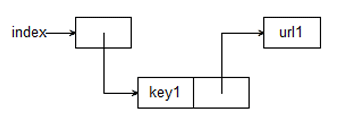
\includegraphics[height=75px, width=200px]{index1.png}
		\caption{Креирање првог поља у индексу}
		\label{slike:indeks1}
		\end{figure}
После иницијалног дела могуће је даље додавати нове листе у индекс, где је почетно поље такође кључна реч (слика \ref{slike:index2}).\\
		\begin{figure}[here]
		\centering
		
		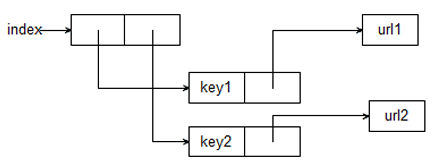
\includegraphics[height=100px, width=260px]{index2.png}
		\caption{Следећа кључна реч и њена хипервеза}
		\label{slike:index2}
		\end{figure}
		Међутим, могуће је да постоји више хипервеза који су везани за исту кључну реч. У том случају, додаје се ново поље листи у којој је та кључна реч (слика \ref{slike:index3}).\\
		\\
		
		\begin{figure}[here]
		\centering
		
		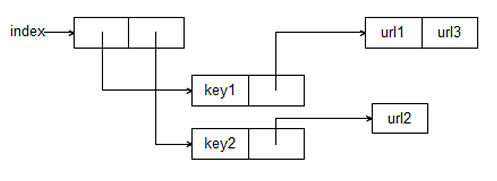
\includegraphics[height=110px, width=300px]{index3.png}
		\caption{Два хиперлинка са истом кључном речју}
		\label{slike:index3}
		\end{figure}	  
	    За прављење и коришћење индекса, потребне су три процедуре:
	    \begin{description}
	    \item[add to index] - процедура која додаје кључну реч и хипервезу у индекс;
	    \item[lookup] - враћа листу свих хипервеза на основу кључне речи;
	    \item[add page to index] - садржај странице (HTML к\^{о}д) раставља на кључне речи и убацује их у индекс.
	    \end{description}
	    У наредним поглављима биће размотрени к\^{о}дови поменутих процедура.
		\subsubsection{Прављење индексa}
		Процедура додавања кључних речи и хипервеза у индекс, узима три податка: index (листа) и две ниске - кључну реч (keyword) и хипервезу(url).
		\begin{lstlisting}[caption=Процедура add\_to\_index, label={lst:addtoindex}, numbers=left]
def add_to_index(index, keyword, url):
    for entry in index:
        if entry[0]==keyword:
            entry[1].append(url)
            return  # ne vraca se nista, samo se menja index
    index.append([keyword, [url]])
		\end{lstlisting}
		Ова процедура прелистава индекс и ако наиђе кључна реч која постоји у индексу, онда само додаје нову хипервезу у листу хипервеза, а ако кључна реч не постоји у индексу, додаје нову листу у индекс, са једном хипервезом.
		\subsubsection{Процедура за претраживање индекса}
		Процедура тражења узима два податка: index (листа) и кључну реч (ниска).
		\begin{lstlisting}[caption=Процедура lookup, label={lst:lookup}, numbers=left]
def lookup(index, keyword):
    lookup_list = []
    for entry in index:
        if entry[0]==keyword:
            for entry_url in entry[1]:
                lookup_list.append(entry_url)
    return lookup_list  
		\end{lstlisting}
		Процедура прво прави привремену листу и претражује индекс, тражећи кључну реч. Када је нађе, онда сваку хипервезу везану за ту кључну реч, поставља у привремену листу и њу враћа као резултат.
		\pagebreak
		\subsubsection{Градња индекс листе}
		Сад кад је позната процедурa add\_to\_index, могуће је дати к\^{о}д процедуре add\_page\_to\_index, која узима три варијабле: индекс листу, хипервезу као ниску и садржај странице такође као ниску. Ова процедура служи за прављење индекса. 
		\begin{lstlisting}[caption=Процедура add\_page\_to\_index , label={lst:addpagetoindex}, numbers=left]
def add_page_to_index(index, url, content):
    for entry in content.split():
        add_to_index(index, entry, url)
		\end{lstlisting}
		Процедура читав садржај странице раставља на речи (празан карактер је подразумевана вредност за сепаратор) и онда се сваку реч додаје у индекс заједно са хипервезом. 
		\subsubsection{Промена веб-паука да ради са индексом}
		Пошто су наведене ове три кључне процедуре к\^{о}д измењеног веб-паука тако да ради са индексом. 
		
	    \begin{lstlisting}[caption=Веб-паук који ради са индексом, label={lst:crawler}, numbers=left]
def get_page(url):
    try:
        import urllib
        return urllib.urlopen(url).read()
    except:
        return ""
def union(a, b):
    for e in b:
        if e not in a:
             a.append(e)
def get_next_target(page):
    start_link = page.find('<a href=')
    if start_link == -1:
        return None, 0
    start_quote = page.find('"', start_link)
    end_quote = page.find('"', start_quote + 1)
    url = page[star_quote + 1: end_quote]
    return url, end_quote
def get_all_pages(page):
    while True:
        links = []
        url, endpos = get_next_target(page)
        if url:
            links.append(url)
            page = page[endpos:]
        else:
            break
    return links

# kreiranje indexa

def add_to_index(index, keyword, url):
    for entry in index:
        if entry[0] == keyword:
            entry[1].append(url)
            return
    index.append([keyword, [url]])
def add_page_index(index, url, content):
    for entry in content.split():
        add_to_index(index, entry, url)

# glavna funkcija

def crawl_web(seed):
    tocrawl = [seed]
    crawled = []
    index = [] # inicijalizacija indexa
    while tocrawl:
        page = tocrawl.pop()
        if page not in crawled:
            content = get_page(page)
            add_page_to_index(index, page, content)
            union(tocrawl, get_all_pages(content))
            crawled.append(page)
    return crawled
    \end{lstlisting}
    Ако се овом  к\^{о}ду придода и к\^{о}д процедуре \emph{lookup}, онда се добијају резултати у облику листе свих хипервеза које одговарају траженој кључној речи. Следи дата процедура која ради са индексом: 
    \begin{lstlisting}[caption=Процедура lookup која ради са индексом, label={lst:lookup_index}, numbers=left]
def lookup(index,keyword):
    lookup_list = []
    for entry in index:
        if entry[0]==keyword:
            for entry_url in entry[1]:
                lookup_list.append(entry_url)
    return lookup_list
    \end{lstlisting}
    Већ сад је могуће добити све хипервезе у односу на тражену кључну реч. За резултате погледати поглавље \ref{sec:dodatakb}.
    \pagebreak
	\subsection{Како убрзати?}
	У претходним поглављима овог рада је изграђен систем који може да одговори на упите, тако што ће проверити једну кључну реч из индекса у једном тренутку. Претраживач ће преко \textbf{lookup} процедуре проверити да ли у индексу постоји кључна реч која је постављена у упит и онда на основу тога дати одговарајући резултат. \\
	Ипак, са великим индексом и већим бројем упита, овакав систем ће се испоставити као \emph{спор}. Типични претраживач би требало да одговори на упите за мање од секунде, ако не и много брже. Закључак је да претраживач мора да ради брже са великим индексом.\\
	Поставља се питање шта је потребно да би неки програм боље радио, одн. узимао што мање ресурса, а у исто време што брже достављао тражене резултате. Наравно, при томе не сме да се доведе у питање тачност и квалитет рада. Када програми постану велики, потребно је водити рачуна о томе колико "коштају" када их покренемо. Евалуација трошкова једног програма приликом његовог рада, је веома важна и представља један од највећих проблема у рачунарству. Поступак евалуације се назива \emph{анализа алгоритма}\index{algoritam@алгоритам!analiza algoritma@анализа алгоритма}\footnote{Под алгоритмом подразумевамо било коју добро дефинисану процедуру која узима неку вредност или скуп вредности као \emph{улаз} и као резултат даје неку вредност или скуп вредности као \emph{излаз}\cite{cormen2001introduction}}\\
	Цена алгоритма зависи од улаза. Цена се касније испоставља у већој потрошњи ресурса рачунара. Претпоставимо да имамо два различита алгоритма Алго1 и Алго2, који успешно решавају исти проблем:
	\begin{itemize}
	\item Улаз $\longrightarrow$ Алго1 $\longrightarrow$ Резултат
	\item Улаз $\longrightarrow$ Алго2 $\longrightarrow$ Резултат
	\end{itemize}
	Није могуће поставити фиксну цену и рећи конкретну суму колико коштају сваки од ова два алгоритма. За неке улазе, Алго1 ће бити јефтинији него Алго2, али за друге улазе, ситуација ће бити другачија. Другим речима, потребно је предвидети цену, а да се не анализира алгоритам за сваки улаз. \\
	Количина улазних података је главни фактор који утиче на брзину алгоритма, одн. цена извршења програма је директно пропорционална односа између повећања улазних података и повећања времена које је потребно да се изврши програм. \\
	Дакле, потребно је знати која је цена (време, меморија) извршења једног програма у зависности од количине улазних података. Такође, потребно је посебно анализирати најгору могућу ситуацију приликом процеса претраживања. Са  \textbf{lookup} процедуром и индексом чији к\^{о}д је наведен у претходном поглављу, најгори случај би био ако се кључна реч која се тражи у упиту налази на крају индекс листе. Тако да, независно од количине улазних података (индекс), не може се са сигурношћу предвидедти колико ће времена требати док се добије резултат, јер кључна реч може да се нађе одмах на почетку листе, где би се резултат добио готово одмах, али може и да се нађе на крају индекс листе, где је потребно претражити све елементе листе.\\
	 	
		\subsubsection{Хеш табела}
		Уколико редослед елемената није битан, може се користити колекција која обезбеђује много бржи приступ елементима. Таква структура се назива хеш табела. Она организује елементе по сопственом редоследу. Наиме, сваки елемент добија свој број, хеш-к\^{о}д, који не зависи од осталих елемената. Битно је да се хеш-к\^{о}д брзо израчуна и да то израчунавање зависи само од елемента који се смешта у хеш табелу. \\
		Хеш табела се реализује као низ листи (или мапа). За проналажење и смештање елемента у хеш табелу израчунава се хеш-к\^{о}д. Резултат је индекс члана у низу, тј. индекс листе у коју ће бити смештен или која садржи дати елемент. Ако нема других елемената у тој листи, онда се елемент смешта на прво место у датој листи. Ако дође до тзв. \emph{колизије}, тј. ако већ постоји елемент и/или више елемената у тој листи, тада се нови елемент пореди са осталима из дате листе и ако га већ нема у листи, додаје се на крај листе.\\
		\begin{figure}[here]
		\centering
		
		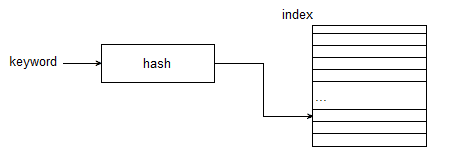
\includegraphics[height=162px, width=472px]{hashtab1.png}
		\caption{Хеш табела}
		\label{slike:hash1}
		\end{figure}
		
		 \begin{figure}[here]
		 \centering
		
		 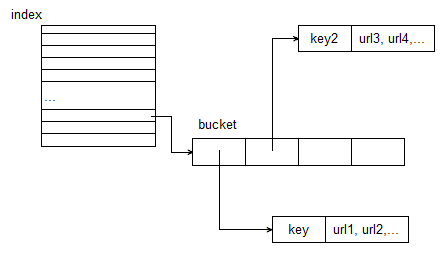
\includegraphics[height=257px, width=446px]{hashtab2.png}
		 \caption{Смештање елемената у листу хеш табеле}
		 \label{slike:hash2}
		 \end{figure}
		Дакле, ако постоје \emph{k} кључних речи и \emph{b} листа у хеш табели, потребно је имати одговарајућу процедуру која ће смештати кључну реч у одговарајућу листу. \\
		
		\subsubsection{Дефинисање хеш функције}
		Претпоставимо да имамо \emph{b} листи у хеш табели. Хеш функција треба да узме као улазне податке кључну реч и број листи, а да као излаз да вредност између 0 и \emph{b}-1 (слика \ref{slike:hashstring}).\\
		 
		\begin{figure}[here]
		\centering
		
		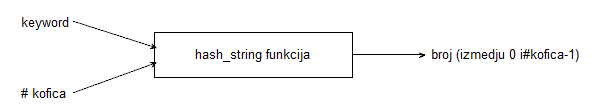
\includegraphics[height=75px, width=400px]{hashstring.png}
		\caption{Hash функција}
		\label{slike:hashstring}
		\end{figure} 
		Најједноставније решење би било да функција узима прво слово кључне речи, налази \emph{ASCII}\index{ASCII@\emph{ASCII}}\footnote{скраћеница од „Амерички стандардни код за размену података“ (енгл. \emph{American Standard Code for Information Interchange}) је кодни распоред заснован на латиничном писму које се користи у енглеском језику. Сваки карактер добија одговарајући број. На пример. "а" има број 98, "А" 67, "б" 99, итд.} кодни број карактера који је прво слово кључне речи, затим дели тај број по модулу \emph{b} (где је \emph{b} број листи хеш табеле) и резултат тог дељења даје индексни број листе у коју ће кључна реч бити смештена.
		\begin{lstlisting}[caption = "Лоша" хеш функција, label = {lst:badhash}, numbers = left]
def bad_hash_string (keyword, buckets):
    return ord(keyword[0]%buckets)
		\end{lstlisting}
		Да би се анализирало да ли је ово добар начин да се равномерно поделе кључне речи по листама у табели, потребно је тестирати ову функцију\index{hash!hash funkcija@хеш функција}. Следећа функција ће послужити да би се видела расподела елемената по листама хеш табеле:
		\begin{lstlisting}[caption = Тестирање хеш функције, label={lst:hashtest}, numbers=left]
def test_hash_function(func, keys, size):
   results = [0] * size  
   keys_used = []
   for w in keys:
       if w not in keys_used:
           hv = func(w, size)
           results[hv] += 1
           keys_used.append(w)
   return results
		\end{lstlisting}
		\pagebreak
		Ова функција ће узети као улазне податке саму хеш функцију, кључне речи (као листу ниски) и број листи хеш табеле. Резултат који се добија није најбољи:
		\begin{lstlisting}[caption = Резултат тестирања лоше hash функције, label={lst:resultstest}]
words = get_page('http://www.gutenberg.org/files/1497/1497.txt').split()
# uzimaju se sve reci iz Platonove "Republike"

counts = test_hash_function(bad_hash_string, words, 12)
# rezultat testiranja se smesta u promenljivu counts

print counts
[725, 1509, 1066, 1622, 1764, 834, 1457, 2065, 1398, 750, 1045, 935]
		\end{lstlisting}
		Као што се види, у једној листи имамо 725 речи, а у другој преко 2000. То није добро, јер је циљ распоредити речи што уједначеније, а тиме и убрзати процес тражења кључних речи у хеш табели.\\
Бољи начин прављења хеш функције био би да се зависно од кључне речи, саберу ASCII к\^{о}дови свих знакова у тој речи, затим се тај збир подели по модулу броја листи хеш табеле и резултат дељења ће бити индексни број листе у коју се смешта кључна реч. 
        \begin{lstlisting}[caption=Боља хеш функција, label={lst:betterhash}, numbers = left]
def hash_string(keyword, buckets):
    h = 0
    for c in keyword:
        h = (h + ord(c))%buckets
    return h 
        \end{lstlisting}
        Ако се тестира нова хеш функција\index{hash!hash funkcija@hash функција} за исте улазне вредности, резултати ће бити нешто бољи:
        \begin{lstlisting}[caption = Тестирање "боље" хеш функције,label={lst:betterhashtest}]
counts = test_hash_function(hash_string, words, 12) 
# rezultat testiranja nove funkcije
[1363, 1235, 1252, 1257, 1285, 1256, 1219, 1252, 1290, 1241, 1217, 1303]
        \end{lstlisting}
        Очигледно је расподела боља, мада свакако није идеална. Најмање попуњена листа има 1217 речи, а највише преко 1360. Тражење идеалне расподеле је предмет шире расправе, тако да ће за потребе овог рада, бити усвојена ова функција као пример добре расподеле. 
        \pagebreak	
		\subsubsection{Прављење празне хеш табеле}
		Ако је познат број листа хеш табеле, потребно је прво направити празну хеш табелу у коју ће се касније смештати подаци. Питање је какву структуру одабрати за ову табелу\index{hash!hash tabela@hash табела}. Следи к\^{о}д који прави празну хеш табелу од \emph{n} листи. 
		\begin{lstlisting}[caption=Празна хеш табела, label={lst:emptyhash}, numbers = left]
def make_hashtable(n):
    i = 0
    table = []
    while i < n:
        table.append([])
        i = i + 1
    return table
		\end{lstlisting}
		
		\subsubsection{Налажење одговарајуће листе}
		Ако је потребно сместити податке у листе хеш табеле, онда мора бити познат индексни број листе у коју ће се сместити податак. Такође, кад се укаже потреба за  претраживањем података, опет мора бити познат индексни број листе у којој се налази тражени елемент. Дакле, потребне су две процедуре, нпр. \emph{add} и \emph{lookup}, прва која ће да додаје елементе у хеш табелу, а друга која ће да тражи одговарајући податак у табели. Претпоставимо да већ постоје функције \emph{hash\_string}(видети к\^{о}д \ref{lst:betterhash}) и \emph{make\_hashtable}(видети к\^{о}д \ref{lst:emptyhash}) које су раније наведене. 
		\begin{lstlisting}[caption= \emph{add} и \emph{lookup} функције, label={lst:addlookup}, numbers = left]
# pomocna funkcija: vraca indeksni broj liste u odnosu na keyword
def hashtable_get_bucket(htable, keyword):
    return htable[hash_string(keyword, len(htable))]


# funkcija dodavanja u tabelu
def hashtable_add(htable, key, value):
    return hashtable_get_bucket(htable, key).append([key, value])


# funkcija trazenja
def hashtable_lookup(htable, key):
    bucket = hashtable_get_bucket(htable, key)
    for i in bucket:
        if i[0]==key:
            return i[1]
    return None
		\end{lstlisting}
		На почетку наведеног к\^{о}да је дата помоћна функција \emph{hashtable\_get\_bucket} јер се употребљава у обе тражене функције за исту сврху - враћање индексног броја листе за одговарајућу кључну реч. 
		\subsubsection{Коришћење мапе уместо листе}
		Уместо листе за прављење хеш табеле, могуће је користити мапе (погледати под \ref{subsec:maps}). Да би се имплементирала таква структура, потребно је преправити претходно наведене процедуре: \textbf{crawl\_web}, \textbf{add\_to\_index} и \textbf{lookup}, тако да могу да раде са мапама, а не са листама. Предност мапа у односу на листе је прегледност и бржи рад. Тако да би алгоритам могао да буде реализован на следећи начин: 
		\begin{lstlisting}[caption=Мапа уместо листе, label={lst:dictionary}, numbers=left]
def get_page(url):
    try:
        import urllib
        return urllib.urlopen(url).read()
    except:
        return ""

def union(p,q):
    for e in q:
        if e not in p:
            p.append(e)
            
def get_next_target(page):
    start_link = page.find('<a href=')
    if start_link == -1:
        return None, 0
    start_quote = page.find('"', start_link)
    end_quote = page.find('"', start_quote + 1)
    url = page[start_quote + 1:end_quote]
    return url, end_quote

def get_all_pages(page):
    while True:
        links = []
        url, endpos = get_next_target(page)
        if url:
            links.append(url)
            page = page[endpos:]
        else:
            break
    return links

# index
def add_to_index(index,keyword,url):
    if keyword in index:
        index[keyword].append(url)
    else:
        index[keyword]=[url]

def add_page_to_index(index,url,content):
    for entry in content.split():
        add_to_index(index, entry, url)
        
# lookup
def lookup(index, keyword):
    if keyword in index:
        return index[keyword]
    else:
        return None


def crawl_web(seed):
    tocrawl = [seed]
    crawled = []
    index = {} #inicijalizacija mape
    while tocrawl:
        page = tocrawl.pop()
        if page not in crawled:
            content = get_page(page) 
            add_page_to_index(index, page, content)
            union(tocrawl, get_all_pages(content))
            crawled.append(page)
    return crawled		
		\end{lstlisting}
		\pagebreak
	\section{Рангирање страница}
	Пошто је завршен к\^{о}д \emph{crawl\_web} процедуре и када постоји веб-паук који може на задовољавајући начин да скенира странице, смешта линкове у индекс или хеш табелу и да даје резултате у односу на постављене упите, следећи корак је рангирање страница. Рангирање страница је и најзахтевнији део веб претраживача. На почетку поглавља је поменут алгоритам за рангирање страница \emph{PageRank}$^tm$\index{PageRank@\emph{PageRank}}, који је срце Гугловог претраживача. У оквиру овог рада реализоваће се алгоритам сличан \emph{PageRank}$^tm$ алгоритму у Python програмском језику. 
		\subsection{Такмичење у популарности}
		Поставља се питање: ко је популаран? Шта је популарност\index{PageRank@\emph{PageRank}!popularnost@популарност}? Ако Ана има највише пријатеља да ли је она најпопуларнија? У школи, на пример, није најважније имати пуно пријатеља, поготово ако су ти пријатељи особе које немају много пријатеља. Важно је и да пријатељи буду популарни. Такође, треба имати у виду и да особа која има јако пуно пријатеља то пријатељство баш и не цени, те тиме и популарност опада.\\
		Теза оснивача Гугла, Брина и Пејџа, каже\cite[Ch 4]{langville2011google} \begin{quote}
		\textit{Страница је важна ако се на њу показује са других важних страница.}
		\end{quote}
		Прва верзија формуле за израчунавање популарности у PageRank алгоритму је сличила следећем:
		\begin{equation}\label{eq:rank1}
		rank(P_{i})=\sum_{P_{j}\in B_{P_{i}}}\frac{rank(P_{j})}{\left |P_{j}  \right |}
		\end{equation}
		где је $P_{i}$ $i$-та страница, $B_{P_{j}}$ скуп страна које показују на $P_{ј}$, $\left |P_{j}  \right |$ број излазних линкова од $P_{j}$. Проблем са формулом \ref{eq:rank1} је у томе што не може да се одреди број $P_{j}$, одн. број линкова од $P_{j}$ ка $P_{i}$. Проблем је решен коришћењем итеративне методе. Дакле, у почетку све странице имају ранг $\frac{1}{n}$, где је $n$, број страница у Гугловом индексу. Тако да се сада рачуна сваки $rank(P_{i})$ за сваку страницу $P_{i}$ из индекса и онда само треба одредити после колико итерација $k$ ће $rank_{k+1}(P_{i})$ бити довољно прецизан. Тако да формула гласи\cite[Ch 4.1]{langville2011google}
		\begin{equation}\label{eq:rank2}
		rank_{k+1}(P_{i})=\sum_{P_{j}\in B_{P{j}}}\frac{rank_{k}(P_{j})}{\left |P_{j}  \right |}
		\end{equation}
		где је $rank_{0}(P_{i})=\frac{1}{n}$ за сваку страницу из индекса.\\
		На пример, ако се претпостави да постоји овакав оријентисан граф\index{graf@граф} на слици \ref{slike:graf}, који представља модел четири веб странице, где су хипервезе представљане уређеним везама. 
		\begin{figure}[here]
		\centering
		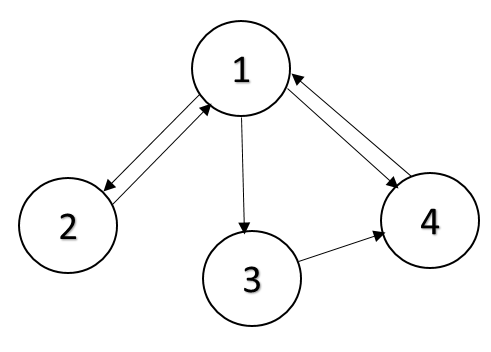
\includegraphics[scale=0.6]{graf.png}
		\caption{Оријентисани граф модела четири веб странице}
		\label{slike:graf}
		\end{figure}
		
		Израчунавање ранга\index{PageRank@\emph{PageRank}!rang@ранг} у две итерације је представљано у табели \ref{tabele:rank}.
		\begin{table}[h]
		
		\centering
		\def\arraystretch{1.5}
		\begin{tabular}{|c|c|c|c|}\hline
		\textbf{итерација 0} & \textbf{итерација 1} & \textbf{итерација 1} & \textbf{PageRank}\\ \hline\hline
		$rank(1)=\frac{1}{4}$ & $\frac{1}{2}$ & $\frac{5}{12}$ & \textrm{I} \\ \hline
		$rank(2)=\frac{1}{4}$ & $\frac{1}{12}$ & $\frac{1}{6}$ & \textrm{III} \\ \hline
		$rank(3)=\frac{1}{4}$ & $\frac{1}{12}$ & $\frac{1}{6}$ & \textrm{III} \\ \hline
		$rank(4)=\frac{1}{4}$ & $\frac{1}{3}$ & $\frac{1}{4}$ &  \textrm{II}\\ \hline
		\end{tabular}
		
		\caption{Израчунавање PageRank-а у две итерације}
		\label{tabele:rank}
        \end{table}		
        \pagebreak
        \subsection{Матрични облик} 
		Аутори  PageRank-а су заменили суму вектором и од вектора направили матрични модел. Нека је $H$ матрица\index{PageRank@\emph{PageRank}!matrica@матрица} димензија $m\times n$, таква да је $H_{ij}=\frac{1}{\left |P_{i}  \right |}$, ако постоји линк од $i$ ка $j$ или $0$ у супротном. Тада би матрица графа била: 
\[
H=
\begin{blockarray}{ccccc}
& 1 & 2 & 3 & 4  \\
\begin{block}{c(cccc)}
  1 & 0 & \frac{\strut 1}{\strut 3} & \frac{\strut 1}{\strut 3} & \frac{\strut 1}{\strut 3}  \\
  2 & 1 & 0 & 0 & 0  \\
  3 & 0 & 0 & 0 & 1  \\
  4 & 1 & 0 & 0 & 0  \\
\end{block}
\end{blockarray}
 \]
        Нека је $\pi^{T}$ вектор, такав $\pi^{(k)T}$ представља PageRank вектор\index{PageRank@\emph{PageRank}!vektor@вектор} у итерацији $k$. Тада се следећа итерација добија као:
        \begin{equation}
        \pi^{(k+1) T}=\pi^{(k)T}H
        \end{equation}
        Свака итерација захтева једно множење вектора и матрице, што нам даје $O(n^{2})$ израчунавања. Но, како је матрица $H$ са врло мало не-нула поља, она захтева $O(nnz(H))$ израчунавања, где је $nnz(H)$ број ненула елемената матрице $H$. Такође, матрица $H$ веома личи на транзициону стохастичку матрицу\index{Markovljevi lanci@Марковљеви ланци!stohasticka matrica@стохастичка матрица} Марковљевих ланаца\index{Markovljevi lanci@Марковљеви ланци}\footnote{Марковљеви ланци описују стохастичке системе(\emph{стохастичке или вероватносне}, прим. аут.) "без меморије", тј. такве системе код којих вероватноће будућих стања зависе само од садашњег, а не од прошлих стања.\cite{filipovic2006operatori}} тако да је можемо назвати субстохастичком\cite[Ch 4.2]{langville2011google}. Брин и Пејџ нису користили термин "Марковљев ланац". Али оно што јесу урадили је да су матрицу $H$ врло мало модификовали како би она била стохастичка. Уместо термина "Марковљев ланац"\index{Markovljevi lanci@Марковљеви ланци}, користили су термин "случајни сурфер"(енгл. \emph{random surfer})\index{PageRank@\emph{PageRank}!random surfer@\emph{random surfer}}. Када такав сурфер дође на страницу са неколико хипервеза, он бира једну од њих на случајан начин и наставља тај процес унедоглед. У дужем временском периоду, део времена који сурфер\index{PageRank@\emph{PageRank}!random surfer@\emph{random surfer}} проводи на датој веб страници је мерило о релативној важности те странице. Ако он проводи доста времена на некој страници, онда мора да се стално враћа на ту страну. Странице које он поново посећује морају бити важне зато што на њих показују друге важне странице.\\
        Два су главна проблема са иницијалним \emph{случајним сурфером}:
        \begin{description}
        \item[dangling node] овај термин означава чвор графа који не показује ни на један други чвор
        \item[конвергенција] да ли ће и после колико итерације, алгоритам дати исправне и очекиване резултате
        \end{description}
        Као резултат решавања првог проблема, добија се модификована матрица која решава тај проблем, уз помоћ :
        \begin{equation}
        S = H + a(\frac{1}{n}e^{T})
        \end{equation}
        где је $e^T$ јединични вектор, а $a = \left\{\begin{matrix}
1, & dangling\; node \\ 
0, & inace
\end{matrix}\right.$ и $n$ остаје број страница у индексу.\\
        Други проблем, тј. проблем конвергенције, је решен тиме што се матрица $S$ модификовала тако да она постане стохастичка, несводљива, апериодична и примитивна, те тако и конвергира. Модификација матрице $S$ ради се у неколико корака: 
        \begin{equation}
        G = \alpha S + (1-\alpha)\frac{1}{n}ee^{T}
        \end{equation}
        \begin{equation}
        G = \alpha(H + a(\frac{1}{n}e^{T})+(1-\alpha)\frac{1}{n}ee^{T}
        \end{equation}
        \begin{equation}
        G = \alpha H + (\alpha a + (1-\alpha)e)\frac{1}{n}e^{T}
        \end{equation}
        где је $0\leqslant\alpha\leqslant1$ параметар који даје својство \emph{телепортације} случајном сурферу\index{PageRank@\emph{PageRank}!random surfer@\emph{random surfer}}, тј могућност да почне процес из почетка. На пример ако је $\alpha=0.6$ то значи да ће 60\% времена случајни сурфер проводити време кликћући линкове, а 40\% времена ће почињати процес из почетка, бирајући случајним одабиром нову страницу за почетак.\\
        У примеру са слике \ref{slike:graf} после краћег рачунања добија се следећа матрица $G$:
\[G = 
\begin{bmatrix}
0.025 & 0.325 & 0.325 & 0.325 \\ 
0.925 & 0.025 & 0.025 & 0.025 \\ 
0.025 & 0.025 & 0.025 & 0.925 \\ 
0.925 & 0.025 & 0.025 & 0.025
\end{bmatrix}
\]
\pagebreak
       \subsection{Израчунавање вредности PageRank\texttrademark{} вектора}
       Вектор $\pi^{T}$\index{PageRank@\emph{PageRank}!vektor@вектор} је могуће добити на два начина, уз услов да је $\pi^{T}e = 1$:
       \begin{enumerate}
       \item Налажењем леве сопствене вредности матрице\index{sopstvene vrednosti matrice@сопствене вредности матрице} $G$, тј $\pi^{T}G=\lambda \pi^{T}$
       \item Налажењем левог нула вектора од $I - G$, тј. $\pi^{T}(I-G)=O^{T}$
       \end{enumerate}
       У примеру са слике \ref{slike:graf} добија се: $\pi^{T} = \left [0.7608\: 0.2740\: 0.2740\: 0.5206 \right ]$\footnote{Израчунато у Python-у, помоћу модула numpy\index{numpy@\emph{numpy}} - \texttt{www.numpy.org} и scypy\index{scypy@\emph{scypy}} \texttt{www.scypy.org}} 
       \begin{lstlisting}[caption=Израчунавање леве сопствене вредности, label={lst:eigen}, numbers=left]
import numpy as np
from scipy.linalg import eig

T = np.mat("0.025 0.325 0.325 0.325;
            0.925 0.025 0.025 0.025; 
            0.025 0.025 0.025 0.925; 
            0.925 0.025 0.025 0.025")
            
values, left = eig(T, left = True, right = False)

for i in range(len(values)):
	print("Levi sopstveni vektor za sopstvenu vrednost {}:".format(values[i]))
	print(left[:,i])
	print()
>>>Levi sopstveni vektor za sopstvenu vrednost (0.9999999999999998+0j):
[-0.76083506+0.j -0.27398492+0.j -0.27398492+0.j -0.52057136+0.j]
        \end{lstlisting}
        Тумачећи резултате, долази се до закључка да је страница \textbf{1} најпопуларнија, јер има највећу вредност, друга је страница \textbf{4}, а треће место деле странице \textbf{2} и \textbf{3}.
\pagebreak		
		\subsection{Рангирање веб страница у Python-у}
		Имплементација ове варијанте PageRank\index{PageRank@\emph{PageRank}} алгоритма у crawl\_web модул се врши додавањем још једне структуре - граф, како би се знало на који начин је случајни сурфер\index{PageRank@\emph{PageRank}!random surfer@\emph{random surfer}} прегледавао странице. Граф\index{graf@граф} ће се једноставно иницијализовати у самој функцији crawl\_web, као празна мапа. Граф би требао садржи хипервезу као кључ и листу хипервеза на које показује, као вредност. Тако да измењена функција crawl\_web изгледа овако:
		\begin{lstlisting}[caption=Увођење графа у crawl\_web, label={lst:graph}, numbers=left]
def crawl_web(seed):
    tocrawl = [seed]
    crawled = []
    graph = {}  # <url>, [lista stranica na koje pokazuje]
    index = {} 
    while tocrawl: 
        page = tocrawl.pop()
        if page not in crawled:
            content = get_page(page)
            add_page_to_index(index, page, content)
            
            outlinks = get_all_links(content)
            graph[page]=outlinks # pravljenje grafa
            
            union(tocrawl, outlinks)
            crawled.append(page)
    return index, graph
		\end{lstlisting}
		\subsection{Израчунавање ранга странице}
		Ранг\index{PageRank@\emph{PageRank}!rang@ранг} странице ће у овом раду бити израчунат помоћу формуле \ref{eq:rank2}, измењену за \emph{dumping} константу, која је позитивна и није већа од 1. Познато је и да је почетна вредност свих страница у нултом кораку итерације иста и изности $\frac{1}{n}$. Дакле,
		\begin{equation}\label{eq:zero}
		rank(0, P_{i})=\frac{1}{n}
		\end{equation}
		\begin{equation}
		rank(k+1, P_{i})=\alpha \sum_{P_{j} \in B_{P_{j}}}\frac{rank(k, P_{j})}{\left |P_{j}  \right |} + (1-\alpha)\frac{1}{n}
		\end{equation}
		Оваква поставка намеће рекурзију\index{rekurzija@рекурзија} као решење, али како није унапред познат број рачунања, тиме је опрезније применити итерацију приликом рачунања. Уз листинг кода \ref{lst:dictionary} и уз измењену функцију crawl\_web из листинга \ref{lst:graph}, сада ће се придодати и функција за израчунавање ранга странице \emph{rank\_compute}, која узима граф као улаз и враћа мапу, чија је кључна реч хипервеза, а вредност је њен ранг.
		\pagebreak
		\begin{lstlisting}[caption=Израчунавање ранга странице, label={lst:rank}, numbers=left]
def compute_ranks(graph):
    alfa = 0.9 # damping faktor
    numloops = 10 # broj iteracija
    
    ranks = {}
    npages = len(graph)
    for page in graph:
        ranks[page] = 1.0 / npages
    
    for i in range(0, numloops):
        newranks = {}
        for page in graph:
            newrank = (1 - alfa) / npages
            
            for node in graph:
                if page in graph[node]:
                    newrank += ranks[node]*alfa/len(graph[node])
            
            newranks[page] = newrank
        ranks = newranks
    return ranks
		\end{lstlisting}
		На крају остаје још да се сортирају резултати и да се омогући кориснику да страницу са највећим рангом види као прву. Ради тога се уводи функција \emph{results}, која ће узети индекс, рангове који су постављени у мапу и наравно, кључну реч корисника. Као резултат се даје листа са свим релевантним хипервезама који су поређани по рангу. 
		\begin{lstlisting}[caption=Функција која враћа најбољи резултат, label={lst:results}, numbers=left]
def results(index, ranks, keyword):
    urls = lookup(index, keyword)
    if urls == None:
        return None
    results_url = []    
    results_num = []
    for e in urls:
        results_num.append(ranks[e])
    results_num.sort()
    while results_num:
        current_max = results_num.pop()
        for url in urls:
            if ranks[url]==current_max:
                results_url.append(url)
                break
    return results_url
      
		\end{lstlisting}
		Овим је у потпуности реализован алгоритам за претраживање веба. К\^{о}д је у целости дат у Додатку А (видети поглавље \ref{sec:dodataka}).
\section{Закључак}
Програмски језик Python поседује разноврстан избор типова података, структура, омогућава програмеру да у кратком временском периоду направи моћан програм. Python поседује све што модеран програмски језик мора да има. Но, он има још више. Армију корисника који учествују у даљем развоју језика својим саветима и расправама на интернет форумима и групама. Python је веома "жив" програмски језик, који периодично избацује нове верзије и побољшава перформансе. \\
		Додаци које Python доноси са својим модулима и проширењима чине га конкурентним у односу на комерцијалне програмске језике какви су Java, C\#...Може се користити и као скрипт језик у оквиру прављења веб апликација, може се користити за писање мањих делова програма у C/C++, а може се користити и самостално за писање десктоп и веб апликација. Данас је незаменљиво оруђе у рукама научника, који га користе за компликоване прорачуне, анализу и презентацију података. \\
		Проширење у виду $django$\index{Python!django@\emph{django}} \emph{framework}-а\footnote{погледати \texttt{http://www.djangoproject.com/}} омогућава широку употребу Python-а у писању веб апликација, пре свега CMS\footnote{Content Management System}, али и мањих веб страница. \\
		Програмски језик Python у овом раду је у потпуности одговорио на потребе писања веб претраживача. Током писања к\^{о}да, коришћене су само основне функције Python-а. Нису се употребљавале компликоване и робустне структуре, што омогућава потенцијалном читаоцу лак увид у к\^{о}д и процену шта ће к\^{о}д на крају даје као резултат.\\
		Процес који је описан на почетку поглавља \ref{subsec:web} успешно је окончан. Оно што превазилази тему овог рада је даља имплементација веб претраживача у веб апликацији. Међутим, може се закључити да је претраживање са укљученим модулом рангирања далеко подесније, него ли оно које само испоставља списак линкова без претходног рангирања (в. поглавље \ref{sec:dodatakb}).  \\
		Веб претраживање данас је уносан посао. Компаније које нуде услуге веб претраживања наплаћују другим фирмама за резултате својих моћних веб-паукова, као и за трошкове рекламирања, на пример. У модерном добу, где је компанија Гугл оставила штампане енциклопедије на ропотарницу историје, неопходно је имати тачан и поуздан систем веб претраживања. Такође, резултати претраживања сугеришу компанијама на који начин ће лакше доћи до купца. У овом тренутку расте потреба за таквим видом информација. Процес таквог прикупљања информација, назива се \emph{data mining}(енгл., \emph{ископавање података}), где се у процесу сакупљања огромне количине података са Интернета, покушавају донети закључци у циљу бољег функционисања компаније.\\
		На самом крају може се закључити да се предлаже примена језика Python за реализацију алгоритама којим се врши рангирање веб страница. На крају је са успехом имплементиран Python програм за претраживање веба и рангирање страница. 
		\pagebreak
		\section{Додатак А: Завршни к\^{о}д}\label{sec:dodataka}
		Завршни к\^{о}д веб претраживача написан у Python-у:
		\lstinputlisting[caption=Завршни к\^{о}д, label={lst:finalcode}, numbers=left]{crawler.py}
		\pagebreak
		\section{Додатак Б: Резултати}\label{sec:dodatakb}
		Да би се добила слика о значају рангирања страница, направљен је модел четири повезане веб странице, чији је граф дат на слици \ref{slike:graf}. К\^{о}дови страница изгледају овако:\\
		
\begin{lstlisting}[language=HTML, caption=K\^{о}д прве странице, label={lst:prva}, numbers=left]
<html>
<head>
 <title>Prva stranica</title>
 <link rel="stylesheet" href="my.css">
</head>
<body>
 <h1>Prva stranica</h1>
 <ul>
  <li><a href="http://localhost/druga.html">Druga stranica</a></li>
  <li><a href="http://localhost/treca.html">Treca stranica</a></li>
  <li><a href="http://localhost/cetvrta.html">Cetvrta stranica</a></li>
 </ul>
 <p>Prva stranica ima hipervezu ka drugoj stranici, trecoj stranici,
 cetvrtoj stranici. Ova stranica se realizuje u cilju testiranja veb
 pretrazivaca.</p>
</body>
</html>
\end{lstlisting}%
\medskip

\begin{lstlisting}[language=HTML, caption=K\^{о}д друге странице, label={lst:druga}, numbers=left]
<html>
<head>
 <title>Druga stranica</title>
 <link rel="stylesheet" href="my.css">
</head>
<body>
 <h1>Prva stranica</h1>
 <ul>
  <li><a href="http://localhost/prva.html">Prva stranica</a></li>
 </ul>
 <p>Druga stranica ima hipervezu ka prvoj stranici. Ova stranica se realizuje u cilju testiranja veb
 pretrazivaca.</p>
</body>
</html>
\end{lstlisting}%
\medskip
\pagebreak
\begin{lstlisting}[language=HTML, caption=K\^{о}д треће странице, label={lst:treca}, numbers=left]
<html>
<head>
 <title>Treca stranica</title>
 <link rel="stylesheet" href="my.css">
</head>
<body>
 <h1>Treca stranica</h1>
 <ul>
  <li><a href="http://localhost/prva.html">Cetvrta stranica</a></li>
 </ul>
 <p>Treca stranica ima hipervezu ka cetvrtoj stranici. Ova stranica se realizuje u cilju testiranja veb
 pretrazivaca.</p>
</body>
</html>
\end{lstlisting}%
\medskip
\begin{lstlisting}[language=HTML, caption=K\^{о}д четврте странице, label={lst:prva}, numbers=left]
<html>
<head>
 <title>Cetvrta stranica</title>
 <link rel="stylesheet" href="my.css">
</head>
<body>
 <h1>Cetvrta stranica</h1>
 <ul>
  <li><a href="http://localhost/prva.html">Prva stranica</a></li>
 </ul>
 <p>Cetvrta stranica ima hipervezu ka prvoj stranici. Ova stranica se realizuje u cilju testiranja veb
 pretrazivaca.</p>
</body>
</html>
\end{lstlisting}%
\medskip
Странице су затим постављене на локални сервер. Кад се уз к\^{о}д \ref{lst:finalcode} пусти наредба:\\
\lstinline{print(lookup(index, 'stranica')}, добија се следећи резултат:
\begin{lstlisting}
['http://localhost/prva.html',
 'http://localhost/prva.html',
 'http://localhost/cetvrta.html',
 'http://localhost/cetvrta.html',
 'http://localhost/treca.html',
 'http://localhost/treca.html',
 'http://localhost/druga.html',
 'http://localhost/druga.html']
\end{lstlisting}
Очигледно је да обично прегледање без рангирања даје списак свих хипервеза који одговарају датој кључној речи.
\pagebreak
Сада ће уз исти к\^{о}д бити дата наредба:\\
\lstinline{print(compute_ranks(graph))} и тада се добија
\begin{lstlisting}
{'http://localhost/treca.html': 0.1572993996378601,
 'http://localhost/cetvrta.html': 0.28313891934814817,
 'http://localhost/prva.html': 0.40226228137613174,
 'http://localhost/druga.html': 0.1572993996378601}
\end{lstlisting}
У овом случају, испоставља се мапа у којој су кључеви хипервезе, а вредности њихов ранг у моделу.\\
Ако је потребно поређати хипервезе по редоследу рангирања, онда се наредбом:\\
\lstinline{print(rank_list(compute_graph(graph)))}, добија листа\\
\begin{lstlisting}
['http://localhost/prva.html',
 'http://localhost/cetvrta.html',
 'http://localhost/treca.html',
 'http://localhost/druga.html']
\end{lstlisting}
И за сам крај, могуће је доставити кориснику тачно једну хипервезу, која одговара упиту и која има највећи ранг од свих хипервеза које одговарају упиту.\\
\lstinline{print(lucky_search(index, compute_ranks(graph), 'stranica'))}, тако да је резултат само прва страница.
\begin{lstlisting}
http://localhost/prva.html
\end{lstlisting}

Може се извући закључак да је далеко корисније претраживање са укљученим модулом рангирања, које омогућава кориснику да за свој задати упит добије као резултат једну или више рангираних страница и тиме добије адекватну информацију. 


		\pagebreak
		\section{Додатак В: Списак програмских к\^{о}дова употребљених у раду}
		Следи списак к\^{о}дова који су коришћени у овом раду.
		\lstlistoflistings
		
		\pagebreak
		
		\bibliography{master}
	    \bibliographystyle{plain}
	    \addcontentsline{toc}{section}{Литература}
	    %\printindex
	    %\printbibliography


\end{document}
